\documentclass[12pt]{article}

\usepackage[numbers, compress]{natbib}
\usepackage[utf8]{inputenc} % allow utf-8 input
\usepackage{hyperref}       % hyperlinks
\usepackage{url}            % simple URL typesetting
\usepackage{booktabs}       % professional-quality tables
\usepackage{amsfonts}       % blackboard math symbols
\usepackage{nicefrac}       % compact symbols for 1/2, etc.
\usepackage{microtype}      % microtypography
\usepackage{xcolor}         % colors
\usepackage{tikz}
\usetikzlibrary{arrows}
\usepackage{amsmath}
\usepackage{mathtools}
\usepackage{bbm}
\usepackage{amssymb}
\usepackage{algorithm}
\usepackage{algpseudocode}
\usepackage{caption}
\usepackage{subcaption}
\usepackage{graphicx}
\usepackage{float}
\usepackage{placeins}
\usepackage{enumitem}
\usepackage[margin=1in]{geometry}
\usepackage{pdfpages}


%images
\graphicspath{{./img/}}


%bibliography
\bibliographystyle{plainnat}


\title{Inferring community characteristics in labelled networks}

%custom commands
\newcommand{\Xcal}{\mathcal{X}}
\newcommand{\Lcal}{\mathcal{L}}
\newcommand{\Bcal}{\mathcal{B}}
\newcommand{\Gcal}{\mathcal{G}}
\newcommand{\Dcal}{\mathcal{D}}
\newcommand{\Fcal}{\mathcal{F}}
\newcommand{\Vcal}{\mathcal{V}}
\newcommand{\Tcal}{\mathcal{T}}
\newcommand{\Integers}{\mathbb{Z}}
\newcommand{\one}{\mathbbm{1}}
\newcommand{\Gaussian}{\mathcal{N}}
\newcommand{\indep}{\perp \!\!\! \perp}
\newcommand{\specialchoose}{\genfrac{\{}{\}}{0pt}{}}
\newcommand{\Expect}{\mathbb{E}}
\DeclareMathOperator*{\argmax}{arg\,max} % Jan Hlavacek
\DeclareMathOperator*{\argmin}{arg\,min} % Jan Hlavacek



%envs
\newtheorem{definition}{Definition}[section]
\newtheorem{theorem}{Theorem}[section]
\newtheorem{corollary}{Corollary}[theorem]
\newtheorem{lemma}[theorem]{Lemma}


\begin{document}
	
	\pagenumbering{gobble}
	
\includepdf{coversheet}
	\pagenumbering{arabic}
	
	%
	\section*{Technical Abstract}
	Labelled networks form a very common and important class of data,
	naturally appearing in numerous applications in science and engineering.
	A typical inference goal is to determine how the vertex labels
	(called features) affect the network's graph structure. A standard
	approach has been to partition the network into blocks grouped
	by distinct values of the feature of interest. A block-based random
	graph model -- typically a variant of the stochastic block model (SBM) --
	is then used to test for evidence of asymmetric behaviour within these
	feature-based communities. Nevertheless, the resulting communities
	often do not produce a natural partition of the graph. In this work
	we introduce a new generative model, the feature-first block model (FFBM),
	which is more effective at describing vertex-labelled undirected
	graphs and also facilitates the use of richer queries on labelled networks.
	We develop a Bayesian framework for inference with this model,
	and we present a method to efficiently sample from the posterior
	distribution of the FFBM parameters. The FFBM's structure is kept
	deliberately simple to retain easy interpretability of the parameter
	values. We apply the proposed methods to a variety of network data
	to extract the most important features along which the vertices
	are partitioned. The main advantages of the proposed approach are
	that the whole feature-space is used automatically, and features
	can be rank-ordered implicitly according to impact. Any features
	that do not significantly impact the high-level structure can be
	discarded to reduce the problem dimension. In cases where the vertex
	features available do not readily explain the community structure
	in the resulting network, the approach detects this and is protected
	against over-fitting. Results on several real-world datasets
	illustrate the performance of the proposed methods. 
	\clearpage
	\section*{Nomenclature}

We provide a list of frequently used symbols for reference.

\begin{table}[!h]
	\centering
	\caption{Nomenclature}
	\label{tab:nomenclature}
	\begin{tabular}{c|l}
			  Symbol & Meaning \\ \hline
			  $\alpha$ & MH acceptance probability\\
			  $\pi$ & MCMC target probability \\
			  $\phi$ & Softmax activation function \\
			  $\psi$ & SBM parameters excluding $b$ \\
			  $\theta$ & Feature-to-block generator parameters \\
			  $\xi$ & Injected noise term in MALA\\
			  $A$ & Graph adjacency matrix \\
			  $b$ & Block membership vector\\
			  $B$ & Total number of blocks \\
			  $c$ & Dimensionality reduction cutoff \\
			  $D$ & Feature-space dimension \\
			  $e$ & Inter-block edge count matrix \\
			  $E$ & Total number of edges \\
			  $f$ & Fraction of vertices kept for training set\\
			  $k$ & Degree sequence or standard deviation multiplier\\
			  $\Lcal$ & Average cross-entropy loss\\
			  $N$ & Number of nodes in graph \\
			  $q$ & MH proposal distribution\\
			  $S$ & SBM description length\\
			  $T$ & Length of Markov chain\\
			  $\Tcal$ & Retained sample set\\
			  $U$ & Negative log-posterior for $\theta$ \\
			  $w$ & Softmax weight vector\\
			  $x$ & Feature vector \\
			  $X$ & Feature matrix \\
			  $y$ & Block membership posterior \\
	\end{tabular}
\end{table}
	\clearpage
	\tableofcontents
	\clearpage
	
	\section{Introduction}

There is a wealth of networks in the world. Some examples of this graphical data are social networks, website hyperlinks and academic collaboration with more being produced each second. It is clear we need tools to analyse this increasingly omni-present form of data.

A somewhat surprising property of real-world graphs is that they exhibit strong community structure. In other words, each node will often belong to a cluster of densely connected nodes. This property is often exploited by graph compression algorithms and there is high interest in recovering the communities from the observed graph.

A common subset of graphical data is the labelled network. This is a graph where we have information about the properties of each node. We shall refer to these node properties as features. One of the most common questions we can ask of this dataset is what features have the largest impact on the structure of the graph. For example, when analysing an academic collaboration graph, one may wish to ask what impact gender has on the structure of the network.  Nevertheless, this analysis is often vulnerable to confounding variables. While gender very well may impact the structure of the graph, there is often a better explanatory variable for the structure.

There is space to bridge the gap between these two approaches. Rather than determining whether a feature impacts the graphical structure directly, we can use the community concept as a stepping stone in our analysis. Therefore, we extract which features have the largest impact on overall graphical structure. This can be thought of as a form of dimensionality-reduction where we only keep the node features that are useful in predicting community memberships.
	\section{Preliminaries}

We first need a model for community-like structure in a network. For this we adopt the widely-used stochastic block model (SBM). This is a latent variable model where each vertex belongs to a single block and the probability two vertices are connected depends only on the block memberships of each.
Specifically, we will use the microcanonical variant of the SBM, proposed by Peixoto \cite{Peixoto-Bayesian-Microcanonical}. To allow for degree-variability between members of the same block, we adopt the following degree-corrected 
formulation (DC-SBM):
% , defined in~(\ref{defn:microcan-dc-sbm}).

\textbf{Microcanonical DC-SBM} --
Let $N \geq 1$ denote the number of vertices in an undirected graph
with $E$ edges. The block memberships are encoded by a vector $b \in [B]^N$,
where $B$ is the number of non-empty blocks.\footnote{For each integer $K\geq 1$, we use the notation $[K]:=\{1,2,\ldots,K\}$.}
	Let $e=(e_{rs})$ be the $B \times B$ symmetric matrix of edge counts 
between blocks, such that $e_{rs}$ is the number of edges from block $r$ to 
block $s$. 
	Let $k =(k_i)$ denote a vector of length $N$, with $k_i$ being the degree of vertex $i$.

The graph's adjacency matrix $A \in \{0,1\}^{N \times N}$ is generated 
by placing edges uniformly at random, conditional
on the constraints imposed by $b$, $e$ and $k$ being satisfied.
Specifically, if $A \sim \mbox{\rm DC-SBM}_{\rm MC} (b, e, k)$,
then with probability~1 it satisfies,
for all $r,s\in[B]$
and all $i\in[N]$:
%
\begin{equation}
	e_{rs} = \sum_{i, j \in [N]} A_{ij} 
\boldsymbol{1} \{b_i = r\} \boldsymbol{1} \{b_j = s\} 
	\qquad 
	\textrm{and} \qquad
	k_i = \sum_{j \in [N]} A_{ij}.
	\label{eqn:sbm-constraints}
\end{equation}

	\section{Feature-first block model}

In this section we propose a novel generative model for labelled networks. We call this the feature-first block model (FFBM) and outline its structure in \ref{fig:ffbm} As before, we let $N$ denote the number of nodes and $B$ the number of blocks in our graph. We define the vector $x_i \in \Xcal^D$ as the feature vector for the $i$'th vertex. $D$ is the number of features. For the datasets we analyse, we deal with binary feature flags so $\Xcal = \{0, 1\}$. The feature vectors $\{x_i\}_{i=1}^{N}$ may be compactly subsumed into the feature matrix $X \in \Xcal^{N \times D}$.

For the FFBM, we start with the feature matrix X and probabilistically generate a vector of block memberships $b \in [B]^N$. The parameters of this step are encapsulated by $\theta$. Each feature vector $x_i$ is treated independently and used to generate the corresponding block membership $b_i \in [B]$. We choose a single softmax layer to model $p(b_i | x_i, \theta)$. More complex models are possible but then deriving meaning from the inferred parameter distributions is more difficult. Summarising, we write $p(b | X, \theta)$ as follows:
%
\begin{equation}
	p(b| X, \theta) = \prod_{i=1}^{N} p(b_i | x_i, \theta) = \prod_{i=1}^{N} \phi_{b_i} (x_i; \theta)
	= \prod_{i=1}^{N} \frac{\exp\left(w_{b_i}^T x_i\right)}{\sum_{k=1}^{B} \exp \left( w_k^T x_i\right)}
\end{equation}
%
We deliberately exclude a bias term to ensure that the relationships we model are based on features and not information about the size of each detected block; a more complete discussion on this topic is given in \ref{appdx:dimension}. The parameter vector $\theta$ for this stage contains all the weight vectors $\theta = \{w_k\}_{k=1}^{B}$. Each $w_k$ has dimension $D$. We could instead write the parameters $\theta$ as a $B \times D$ matrix of weights $W$; this form has computational benefits as then $z_i \coloneqq W x_i$, which is the input to the softmax activation function.

\begin{figure}[!h]
	\centering
	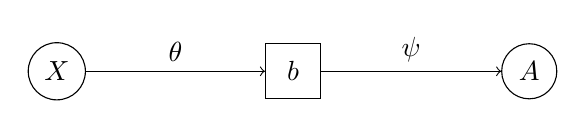
\begin{tikzpicture}[
		roundnode/.style={circle, draw=black, minimum size=7mm},
		squarednode/.style={rectangle, draw=black, minimum size=7mm}
		]
		% nodes
		\node[roundnode] (X) at (0, 0) {$X$};
		\node[squarednode] (b) at (3, 0) {$b$};
		\node[roundnode] (A) at (6, 0) {$A$};
		
		% arrows
		\draw[->] (X.east) -- node[above] {$\theta$} (b.west);
		\draw[->] (b.east) -- node[above] {$\psi$}(A.west);
	\end{tikzpicture}
	\caption{The feature-first block model (FFBM)}
	\label{fig:ffbm}
\end{figure}

Once the block memberships $b$ have been generated, we then draw the graph $A$ from the microcanonical DC-SBM (equation \ref{eqn:A-generation}) with additional parameters encapsulated by $\psi = \{\psi_e, \psi_k\}$.
%
\begin{equation}
	A \sim \textrm{DC-SBM}_{\textrm{MC}} (b, \psi_e, \psi_k)
	\label{eqn:A-generation}
\end{equation}


\subsection{Prior selection}

Before performing any inference, we must specify priors on $\theta$ and $\psi$. For $\theta$ it seems sensible to choose a Gaussian prior, with zero mean and variance matrix $\sigma^2_\theta I$ such that each element of $\theta$ is independent and distributed like $\sim \Gaussian(0, \sigma_\theta^2)$. In vector form, the prior for $\theta$ is therefore:
%
\begin{equation}
	p(\theta) = \Gaussian \left( \theta ; 0, \sigma_\theta^2 I \right)
	\label{eqn:theta-prior}
\end{equation}
%
In our model, the block memberships vector $b$ is an intermediate latent variable and so we are not free to choose a prior for it. Nevertheless, as far as inference on the right-hand-side of figure \ref{fig:ffbm}, we regard $p(b | X)$ as a pseudo-prior on $b$. We can show (appendix \ref{appdx:b|x}) that our choice of prior for $p(\theta)$ in equation \ref{eqn:theta-prior} leads to a uniform $p(b | X)$ in equation \ref{eqn:b-pseudo-prior}.
%
\begin{equation}
	p(b | X) = \int p(b | X, \theta) p(\theta) d\theta = B^{-N}
	\label{eqn:b-pseudo-prior}
\end{equation}
%
This is an enormously important simplification as evaluating $p(b | X)$ does not require an expensive Monte-Carlo integration over the $\theta$-domain nor does it require the exact value of $X$. \citet{Peixoto-Bayesian-Microcanonical} proposes careful choices for the additional microcanonical SBM parameters $\psi$ which we adopt. Peixoto's idea is to write the joint prior on $(b, e, k)$ as a product of conditionals $p(b, e, k) = p(b) p(e | b) p(k | e, b)= p(b) p(\psi | b)$. For our purposes we must insert a conditioning on $X$, to form our pseudo-prior for $b$ and $\psi$, to give equation \ref{eqn:joint-pseudo-prior}.
%
\begin{equation}
	p(b, \psi | X) = p(b | X) p(\psi | b, X) = p(b | X) p(\psi | b)
	\label{eqn:joint-pseudo-prior}
\end{equation}
%
Where we leverage the fact $(\psi \indep X) | b$. We then borrow the priors proposed by \citet{Peixoto-Bayesian-Microcanonical} for $p(\psi | b)$ to complete our model. Please refer to appendix \ref{appdx:sbm} for the exact form of $p(\psi | b)$. All that concerns the main argument is we have a computable form.

	\section{Inference}
\label{sec:inference}

Now that we have defined the FFBM, we wish to leverage it to perform inference. Suppose we are presented with a vertex-labelled graph $(A, X)$; the goal is to draw samples for $\theta$ according to the posterior given the observed data:
%
\begin{equation}
	\label{eqn:theta-target}
	\theta^{(t)} \sim p(\theta | A, X)
\end{equation}
%
However, generating these samples is not easily done in practice. We therefore propose an iterative approach. We first draw samples $b^{(t)}$ from the block membership posterior (equation \ref{eqn:b-samples}) and then use each $b^{(t)}$ to draw samples for $\theta$ as in equation \ref{eqn:theta-samples}. 
%
\begin{align}
	b^{(t)} &\sim p \Big( b | A, X \Big)  \label{eqn:b-samples}\\
	\theta^{(t)} &\sim p\Big(\theta | X, b^{(t)} \Big) \label{eqn:theta-samples}
\end{align}
%
Both of these sampling steps can be implemented with a Markov Chain through the Metropolis-Hastings algorithm \cite{hastings-alg}. We just need to define a proposal distribution $q(x, x')$ for proposing a move $x \rightarrow x'$ and be able to evaluate an un-normalised form of the target distribution, denoted $\pi(\cdot)$, point-wise. The proposed move is then accepted with probability $\alpha$ (equation \ref{eqn:mh-accept}) else it is rejected and we stay at $x$.
%
\begin{equation}
	\alpha(x, x') = \min \left( \frac{\pi(x') q(x', x)}{\pi(x) q(x, x')} , 1 \right)
	\label{eqn:mh-accept}
\end{equation}
%
This accept-reject step ensures the resulting Markov Chain is in detailed balance with the target distribution $\pi(\cdot)$. What we propose in equations \ref{eqn:b-samples} and \ref{eqn:theta-samples} is therefore implemented through a 2-level Markov chain. The resulting samples for $\theta^{(t)}$ are unbiased in the sense that the expectation of their distribution is the posterior we are targetting:
%
\begin{equation}
\Expect_{b^{(t)}} \left[p \left( \theta | X, b^{(t)} \right) \right] = \sum_{b \in [B]^N} p(\theta | X, b) p(b | A, X) = \sum_{b \in [B]^N} p(\theta, b | A, X) = p(\theta | A, X)
\label{eqn:theta-unbiased}
\end{equation}
%
This is an example of a pseudo-marginal approach. Indeed, \citet{pseudo-marginal} show that the unbiased result in equation \ref{eqn:theta-unbiased} is sufficient to prove that for large enough $t$, $\theta^{(t)} \sim \Expect_{b^{(i)}} \left[ p(\theta | X, b^{(t)})\right] = p(\theta 
| A, X)$ which is exactly the distribution we are targetting (equation \ref{eqn:theta-target}).
%
\begin{figure}[!h]
	\centering

	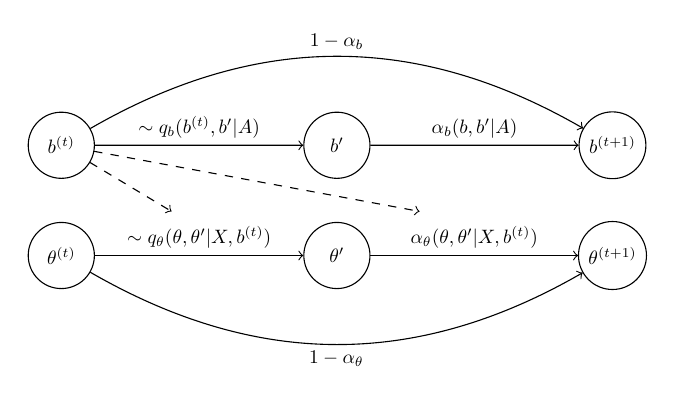
\begin{tikzpicture}[
		scale=0.7, every node/.style={transform shape},
		roundnode/.style={circle, draw=black, minimum size=12mm},
		squarednode/.style={rectangle, draw=black, minimum size=12mm}
		]
		% nodes
		\node[roundnode] (b0) at (0, 2) {$b^{(t)}$};
		\node[roundnode] (b1) at (5, 2) {$b'$};
		\node[roundnode] (b2) at (10, 2) {$b^{(t+1)}$};
		\node[roundnode] (t0) at (0, 0) {$\theta^{(t)}$};
		\node[roundnode] (t1) at (5, 0) {$\theta'$};
		\node[roundnode] (t2) at (10, 0) {$\theta^{(t+1)}$};
		
		% arrows
		\draw[->] (b0) to node[above] {$\sim q_b(b^{(t)}, b' | A)$} (b1);
		\draw[->] (b1) to node[above] {$\alpha_b (b, b' | A)$} (b2);
		\draw[->] (b0) [out=30, in=150] to node[above] {$1-\alpha_b$} (b2);
		
		\draw[->] (t0) to node[above] {$\sim q_\theta(\theta, \theta' | X, b^{(t)})$} (t1);
		\draw[->] (t1) to node[above] {$\alpha_\theta (\theta, \theta' | X, b^{(t)})$} (t2);
		\draw[->] (t0) [out=-30, in=-150] to node[below] {$1-\alpha_\theta$} (t2);
		
		\draw[dashed, ->] (b0) to (2, 0.8);
		\draw[dashed, ->] (b0) to (6.5, 0.8);
		
	\end{tikzpicture}
	\caption{Sampling sequence}
	\label{fig:samp-sequence}
\end{figure}

The reason we split the Markov chain into two stages is because the summation over all latent states $b \in [B]^N$ required to directly compute the likelihood $p(A| X, \theta) = \sum_{b \in [B]^N} p(A | b) P(b | X, \theta)$ is intractable -- $O(B^N)$. Figure \ref{fig:samp-sequence} shows an overview of the proposed method. We have introduced subscripts and conditionings to make explicit what variables each step utilises. We note the power of the simplification given by equation \ref{eqn:b-pseudo-prior}. As $p(b| X)$ does not depend on the exact value of X, we do not need to know the value of $X$ to perform the sampling on $b$. Conversely, for the $\theta^{(t)}$ samples, we use only $b^{(t)}$ but not $A$ as $(\theta \indep A) | b$.

\FloatBarrier

\subsection{Sampling block memberships}

\citet{Peixoto-MCMC} proposes a Monte Carlo method which we will base our approach on. It relies on writing the posterior in the following form:
%
\begin{equation}
	p(b | A, X) \propto p(A | b, X) \cdot p(b | X) = \pi_b(b)
\end{equation}
%
Now $\pi_b(\cdot)$ is the un-normalised density we wish to sample from for the $b$-chain. In other words, we wish to construct a Markov chain that has $\pi_b(\cdot)$ as its invariant distribution. We can break $\pi_b$ down as follows:
%
\begin{equation}
	\pi_b(b) = p(b|X) \sum_{\psi} \nolimits p(A , \psi | b, X) \\
	= p(b|X) p(A, \psi^* | b, X) \\
	= p(A | b, \psi^*) \cdot p(\psi^* | b) \cdot p(b | X)
\end{equation}
%
Since we are using the microcanonical SBM formulation, there is only one value of $\psi$ that is compatible with the given $(A, b)$ pair (given in equation \ref{eqn:sbm-constraints}). We denote this value $\psi^* = \{\psi_k^*, \psi_e^*\}$. Therefore, the summation over all $\psi$ reduces to just the single $\psi^*$ term; this is the power of the microcanonical formulation. We also define the microcanonical entropy of the configuration as.
%
\begin{equation}
	S(b) = - \log \pi_b(b) = - \Big( \log p(A | b, \psi^*) + \log p(\psi^*, b | X) \Big)
	\label{eqn:dl-form}
\end{equation}
%
This entropy can equally be thought of as the description length of the graph. The exact form of the proposal $q_b$ is explored thoroughly by \citet{Peixoto-MCMC} and not repeated here. There is a widely used library for Python made available under LGPL called \verb*|graph-tool| \cite{peixoto_graph-tool_2014}, which implements this algorithm. The only modification we make is in the block membership prior $p(b)$ which we replace with $p(b|X)=B^{-N}$, which cancels out in the MH accept-reject step as it is independent of $b$.

\subsection{Sampling feature-to-block generator parameters}

The invariant distribution we wish to target for the $\theta$ samples is the posterior of $\theta$ given the values of the pair $(X, b)$. We write this as follows:
%
\begin{equation}
	\pi_\theta(\theta) \propto p(\theta | X, b) \propto p(b | X, \theta) p(\theta) \propto \pi_\theta (\theta) \propto  \exp \left( - U(\theta) \right)
\end{equation}
%
Where we have introduced $U(\theta)$ equal to the negative log posterior. We define $y_{ij} \coloneqq \one \left\{ b_i = j \right\}$ and $a_{ij} \coloneqq \phi_j(x_i; \theta)$. Discarding constant terms, we can write $U(\theta)$ as in equation \ref{eqn:U-form} (refer to appendix \ref{appdx:form-U} for the derivation).
%
\begin{equation}
	U(\theta) = \left( \sum_{i=1}^{N} \sum_{j=1}^{B} y_{ij} \log \frac{1}{a_{ij}} \right)
	+ \frac{1}{2\sigma_\theta^2} ||\theta||^2 = N \cdot \Lcal(\theta) + \frac{1}{2\sigma_\theta^2} ||\theta||^2
	\label{eqn:U-form}
\end{equation}
%
$U(\theta)$ in equation \ref{eqn:U-form} appears a typical objective function for neural network training. The first term is introduced by the likelihood. We collect it into $N \cdot \Lcal(\theta)$, which is the cross-entropy between the graph-predicted and feature-predicted block memberships summed over all vertices. The second term of equation \ref{eqn:U-form} -- introduced by the prior -- brings a form of regularisation, guarding against over-fitting. Different to traditional applications, our goal is not to find the minimiser of $U(\theta)$ but to draw samples from the posterior $\pi_\theta(\cdot) \propto \exp(-U(\cdot))$. We can use $\nabla U$ as a useful heuristic to bias our proposal towards regions of higher target density. We therefore adopt the Metropolis-adjusted Langevin algorithm (MALA) -- first proposed by \citet{mala-tweedie}. Given the current sample $\theta$, we generate a new sample $\theta'$ according to equation \ref{eqn:theta-update}.
%
\begin{align}
	\theta' &= \theta - h \nabla U(\theta) + \sqrt{2h} \cdot \xi
	\label{eqn:theta-update} \\
	\therefore q_\theta(\theta, \theta') &= \Gaussian \left( \theta' ; \theta - h \nabla U(\theta), 2h I \right)
	\label{eqn:theta-proposal}
\end{align}
%
Where $\xi \sim \Gaussian(0, I)$ and $h$ is a step-size parameter -- which may vary with the sample index (appendix \ref{appdx:step-size} explores this more fully). Without the injected noise term, MALA is equivalent to gradient descent. We require the noise term $\xi$ to fully explore the parameter space. We can write the proposal distribution $q_\theta$ as in equation \ref{eqn:theta-proposal}. The term $\nabla U$ has an easy to compute analytic form (derived in Appendix \ref{appdx:gradu}). By noting that $\theta = \{w_k\}_{k=1}^{B}$, we write the derivative with respect to each $w_k$ as:
%
\begin{equation}
	\frac{\partial U}{\partial w_k} = - \left( \sum_{i=1}^{N} \Big\{ \tilde{x}_i (y_{ik} - a_{ik}) \Big\} - \frac{w_k}{\sigma_\theta^2} \right)
	\label{eqn:U-derivative}
\end{equation}
%
After a proposed move is generated, in typical Metropolis-Hastings fashion we accept the move with probability $\alpha_\theta$, as in equation \ref{eqn:mh-accept}.

\subsection{Sampling sequence}

Up to this point, each $\theta^{(t)}$ update uses its corresponding $b^{(t)}$ sample. This means that the evaluation of $U(\theta)$ and $\nabla U(\theta)$ has high variance. This may lead to longer burn-in for the resulting Markov chain. The only link between $b^{(t)}$ and $\theta^{(t)}$ is in the evaluation of $U(\theta)$ and $\nabla U(\theta)$ which depends only on the matrix $y^{(t)}$ with entries $y_{ij}^{(t)} \coloneqq \one\{b_i^{(t)} = j\}$. We would rather deal with the expectation of each $y_{ij}^{(t)}$:
%
\begin{equation}
	\Expect \left[ y_{ij}^{(t)} \right] = \Expect_{b^{(t)}} \left[ \one(b_{i}^{(t)} = j) \right]
	= p(b_i = j | A, X)
\end{equation}
%
We can obtain an unbiased estimate for this quantity using the set of $b$-samples. However, as with all MCMC methods, we must only uses samples after burn-in and thinning have been applied. We introduce $\Tcal_b$ to denote the retained set of indices for the $b$-samples and $\Tcal_\theta$ similarly for the $\theta$-chain. An in-depth discussion of how these sets are chosen is given in appendix \ref{appdx:burn-in-thinning}. The unbiased estimate for $y_{ij}^{(t)}$ using the restricted sample set $\Tcal_b$ is denoted $\hat{y}_{ij}$ and has form:
%
\begin{equation}
	\hat{y}_{ij} \coloneqq \frac{1}{|\Tcal_b|} \sum_{t \in \Tcal_b} y_{ij}^{(t)} = \frac{1}{|\Tcal_b|} \sum_{t \in \Tcal_b} \one\{b_i^{(t)} = j\}
\end{equation}
%
We choose to feed each $\theta^{(t)}$ update step the same matrix $\hat{y}$ for all $t$ rather than the corresponding $y^{(t)}$. This means we no longer need to run the $b$ and $\theta$ Markov chains concurrently. Instead, we run the $b$-chain to completion and use it to generate $\hat{y}$. This affords us the flexibility to vary the lengths of the $b$ and $\theta$-chains. Furthermore, the changeover from $y^{(t)}$ to $\hat{y}$ reduces the burn-in time for the $\theta$-chain by reducing the variance in our evaluation of $U$ and $\nabla U$. A description of the overall algorithms is given in appendix \ref{appdx:algorithms}.

\subsection{Dimensionality reduction}
\label{sec:dim-reduction}

Once we have the samples $\left\{ \theta^{(t)} \right\} \sim p(\theta | A, X)$, we can compute the empirical mean and standard deviation of each component of $\theta$. Switching back to matrix notation we define $\theta = W$, such that $W_{ij}$ is the weight component for block $i$ and feature $j$, we can define:
%
\begin{equation}
	\hat{\mu}_{ij} \coloneqq \frac{1}{|\Tcal_\theta|} \sum_{t \in \Tcal_\theta} W_{ij}^{(t)} \qquad \textrm{and} \qquad
	\hat{\sigma}_{ij} \coloneqq \frac{1}{|\Tcal_\theta|} \sum_{t \in \Tcal_\theta} \left( W_{ij}^{(t)} - \hat{\mu}_{ij} \right)^2
\end{equation}
%
A simple heuristic to discard the least important features requires specifying a cutoff $c > 0$ and a multiplier $k > 0$. We define the function $\Fcal_i(j)$ as in \ref{eqn:fij} then only keep features with indices $d \in \Dcal'$, where $\Dcal'$ is constructed as in equation \ref{eqn:kept-feature-set}.
%
\begin{align}
	\Fcal_i(j) &\coloneqq (\hat{\mu}_{ij} - k \hat{\sigma}_{ij}, \hat{\mu}_{ij} + k \hat{\sigma}_{ij}) \cap (-c, +c)
	\label{eqn:fij} \\
	\Dcal' &\coloneqq \left\{ j \in [D] : \exists i \in [B] \textrm{ s.t. }  \Fcal_i(j) \neq \emptyset \right\}
	\label{eqn:kept-feature-set}
\end{align}
%
Intuitively, this means discarding any feature for which $\hat{\mu}_{ij} \pm k\hat{\sigma}_{ij}$ lies within or spans the null region $(-c, c)$ for all block indices. If we were to use the Laplace approximation for the posterior $p(W_{ij} | A, X) \approx \Gaussian(W_{ij}; \mu_{ij}, \sigma_{ij})$, then this is effectively a hypothesis test on the value of $W_{ij}$ (equation \ref{eqn:hyp-test-discard}). $\Dcal'$ then comprises all features $i$ for which $H_1$ is accepted at least once for some $j \in [B]$.
%
\begin{equation}
	H_0: |\mu_{ij}| \leq c \qquad
	H_1: |\mu_{ij}| > c
	\label{eqn:hyp-test-discard}
\end{equation}
%
The multiplier $k$ determines the degree of significance of the result. However, as the Laplace approximation is not exact we will only treat this dimensionality reduction method as a useful heuristic and not an exact method. Conversely, we could fix $k=k_0$ and the dimension of our reduced feature set $|\Dcal'|=D'$. We would then like to find the largest value of $c$ such that $|\Dcal'|=D'$ given $k=k_0$. This is summarised in equation \ref{eqn:c-star}. This approach is often preferred as it fixes the number of reduced dimensions.
%
\begin{equation}
	c^* = \argmax_{c>0} (c : |\Dcal'| = D', k=k_0)
	\label{eqn:c-star}
\end{equation}
	\section{Experiments}
\label{sec:experiments}

We apply the outlined methods to a variety of datasets:

\begin{itemize}
	\item \textbf{Political books} \cite{polbooks} ($N=105, E=441, D=3$) -- network of Amazon political book sales, published close to the 2004 presidential election. Two books are connected if they were frequently co-purchased. Vertex features encode the political affiliation of the author (liberal, conservative, or neutral).
	\item \textbf{Primary school dynamic contacts} \cite{schools} ($N=238, E=5539, D=13$) -- network of face-to-face contacts amongst students and teachers at a primary school in Lyon, France. Vertex features include class membership (one of 10 values: 1A-5B), gender (male, female) and teacher status encoded as an 11th school-class. We choose to analyse just the second day of results.
	\item \textbf{Facebook egonet} \cite{fb-snap} ($N=747, E=30025, D=480$) -- an assortment of Facebook users' friends lists. Vertex features are fully anonymised and encode information about each user's education history, languages spoken, gender, home-town, birthday etc. We focus on the egonet with id 1912.
\end{itemize}
%
We first require metrics to assess model performance. We define the average
description length per entity (nodes and edges) $\bar{S}_e$ as a suitable metric to gauge the SBM fit:
%
\begin{equation}
	\bar{S}_e \coloneqq \frac{1}{(N+E) |\Tcal_b|} \sum_{t\in \Tcal_b} S \left( b^{(t)} \right).
	\label{eqn:mean-dl}
\end{equation}

Next, to assess the performance of the feature-to-block predictor, 
we randomly partition the vertex set $[N]$ into training and test sets: $\Gcal_0$ and $\Gcal_1$.
The $b$-chain is run using the whole network but we only use vertices $v \in \Gcal_0$ to train the $\theta$-chain. As $|\Gcal_0| \neq |\Gcal_1|$ in general, we use the average cross-entropy loss 
over each set to gauge fit,
%
\begin{equation}
	\bar{\Lcal}_\star \coloneqq \frac{1}{|\Tcal_\theta|} \sum_{t \in \Tcal_\theta} \Lcal_\star^{(t)},
	\quad \textrm{where} \quad
	\Lcal_\star^{(t)} \coloneqq \frac{1}{|\Gcal_\star|} \sum_{i \in \Gcal_\star}\sum_{j \in [B]} \hat{y}_{ij} \log \frac{1}{\phi_j \left(x_i; \theta^{(t)} \right)},
	\label{eqn:cross-entropy-loss}
\end{equation}
%
where $\star \in \{0, 1\}$ toggles between the training and test sets.
%
Nevertheless, the cross-entropy loss is a coarse measure of fit. We wish to define a new measure of fit specific to each detected block. Let us define
$
	\Bcal_\star(j) \coloneqq \{i \in \Gcal_\star : \hat{b}_i = j\}
$
where
$ 
	\hat{b}_i \coloneqq \argmax_j \hat{y}_{ij}.
$
Now $\Bcal_\star(j)$ is the set of vertices that have maximum a posteriori probability of belonging to block $j$. We now define the accuracy for block $j$ as,
%
\begin{equation}
	\eta_\star(j) \coloneqq \frac{1}{|\Bcal_\star (j)| \cdot 
	|\Tcal_\theta| } 
	\sum_{i \in \Bcal_\star (j)}  \sum_{t \in \Tcal_\theta}
	\one \left\{\hat{b}_i = \argmax_j \phi_j \left( x_i; \theta^{(t)} \right) \right\}.
	\label{eqn:accuracy}
\end{equation}

This effectively tests whether the feature-to-block and the graph-to-block predictions agree in their largest component. We call this metric, $\eta_\star(j)$, the {\em block-accuracy} for block $j$. It is clearly bounded $0 \leq \eta_\star(j) \leq 1$, with an accuracy of 1 meaning perfect agreement for the vertices in detected block $j$.

Table~\ref{tab:results} summarises the results for each experiment. 
We see that the dimensionality reduction procedure 
brings the training and test losses closer together. This implies that 
the features we keep are indeed correlated with the underlying graphical 
partition and that the approach generalises correctly. The test loss variance is higher than the training loss variance as the test set is smaller and so more susceptible to variability in its construction.
%
The average description length per entity,
$\bar{S}_e$, of the graph, 
has very small variance, suggesting that
the detected communities can be found reliably (to within an arbitrary 
relabelling of blocks).

\paragraph{\textbf{Political books.}}

We choose to partition the network into $B=3$ communities as we only have this many distinct values for political affiliation.
From Figure~\ref{fig:polbooks-null} we see that all 3 blocks have a distinct political affiliation as their largest positive component.  
Furthermore, the training and test losses from Table~\ref{tab:results}  
are very similar and both are low in magnitude. This is strong evidence 
that political affiliation is a very appropriate explanatory 
variable for the overall network structure.
%
However, from Figure~\ref{fig:polbooks-accuracy} we see that block 1 has low accuracy. 
This suggests that detected block 1 is not solely composed of ``neutral" books but also 
contains some ``liberal" and ``conservative" authors. Examining 
Figure~\ref{fig:polbooks-graph}, we see the majority of paths between blocks 2 and 3 go through block 1.
Block 1 is in effect a bridge between the ``conservative'' and ``liberal'' blocks so it is unsurprising that some of these leak into block 1.

\paragraph{\textbf{Primary school.}}

We choose the number of communities $B=10$, in line with the total number of 
school classes. Only the pupils' class memberships (1A-5B) survive
the dimensionality-reduction process (Figure~\ref{fig:school-null});
gender and teacher/student status have been discarded,
meaning these are poor predictors of overall macro-structure.
%
The vast majority of blocks are composed of a single class. 
However, some blocks have two comparably strong classes as their predictors (e.g. blocks 2 and 5). 
Conversely, some classes are found to extend over two 
detected blocks (class 2B spans blocks 8 and 9) but we do 
not have a feature which explains the division.
%
Figure~\ref{fig:school-accuracy} shows excellent accuracy for the majority of blocks. In fact the only blocks with low accuracy are those that have a school-class span two blocks such that we cannot reliably distinguish between the two. This is more pronounced when we apply hard classification rather than the soft cross-entropy loss. Perhaps there are unobserved features which explain this divide.

\paragraph{\textbf{Facebook egonet.}}

The retained features 
(Figure~\ref{fig:fb-null}) are those that best explain the high-level 
community structure. The majority of these are education related. 
Nevertheless, for $D'=10$ we only have good explanations for some of the detected blocks; several blocks in 
Figure~\ref{fig:fb-null} do not have high-magnitude components. This is further emphasised by the disparate accuracies in Figure~\ref{fig:fb-accuracy}.
%
For a high-dimensional feature-space, it is likely that a particular
feature may uniquely identify a small set of vertices; if these are all in the same block, then the classifier may overfit despite the penalty imposed by the prior. Indeed, we see in
Figure~\ref{fig:fb-null} that the feature birthday-5 has a very high weight as it relates to block 1 – but it is unlikely that birthdays determine graphical structure.
\begin{table}[!ht]
	\centering
	\caption{Results averaged over $n=10$ iterations (mean $\pm$ std. dev.).}
	\label{tab:results}
	\resizebox{\textwidth}{!}{%
		\begin{tabular}{c|ccc|c|cc|ccc}
			Dataset  & $B$ & $D$ & $D'$ & $\bar{S}_e$ & $\bar{\mathcal{L}}_0$ & $\bar{\mathcal{L}}_1$ & $c^*$ & $\bar{\mathcal{L}}_0'$ & $\bar{\mathcal{L}}_1'$  \\ \hline
			Polbooks & 3 & 3 & -- & $2.250 \pm 0.000$ & $0.563 \pm 0.042$ & $0.595 \pm 0.089$ & -- & -- & -- \\
			School & 10 & 13 & 10 & $1.894 \pm 0.004$ & $0.787 \pm 0.127$ & $0.885 \pm 0.129$ & $1.198 \pm 0.249$ & $0.793 \pm 0.132$ & $0.853 \pm 0.132$ \\
			FB egonet & 10  & 480 & 10 & $1.626 \pm 0.003$ & $1.326 \pm 0.043$ & $1.538 \pm 0.069$ & $0.94 \pm 0.019$ & $1.580 \pm 0.150$ & $1.605 \pm 0.106$
		\end{tabular}
	}
\end{table}

\begin{figure}[!ht]
	\centering
	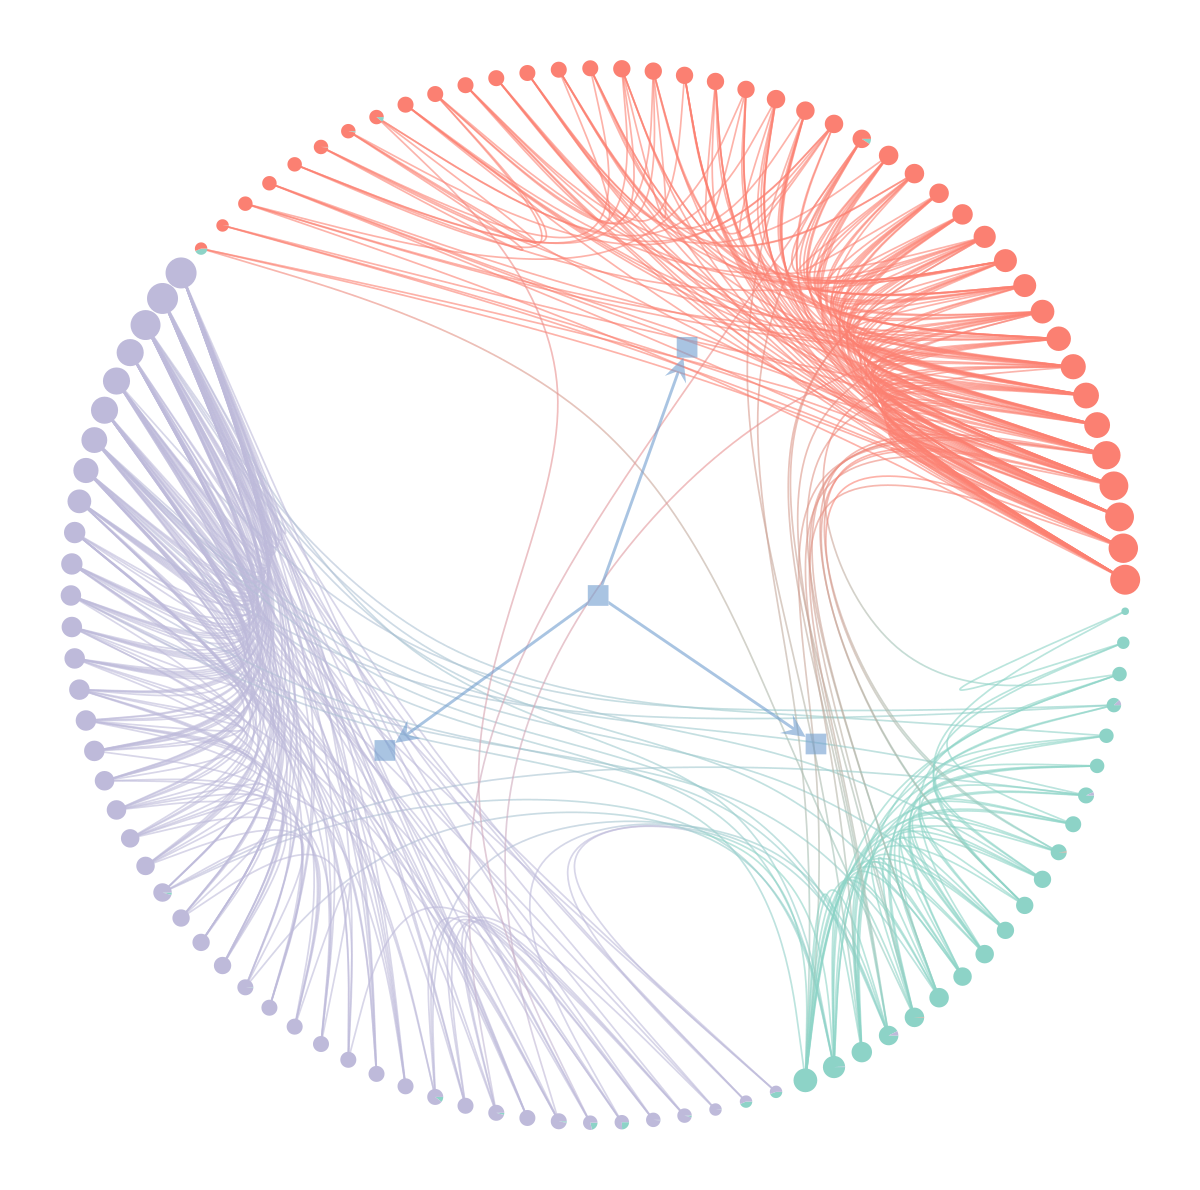
\includegraphics[width=0.28\linewidth]{img/polbooks-graph.png}
	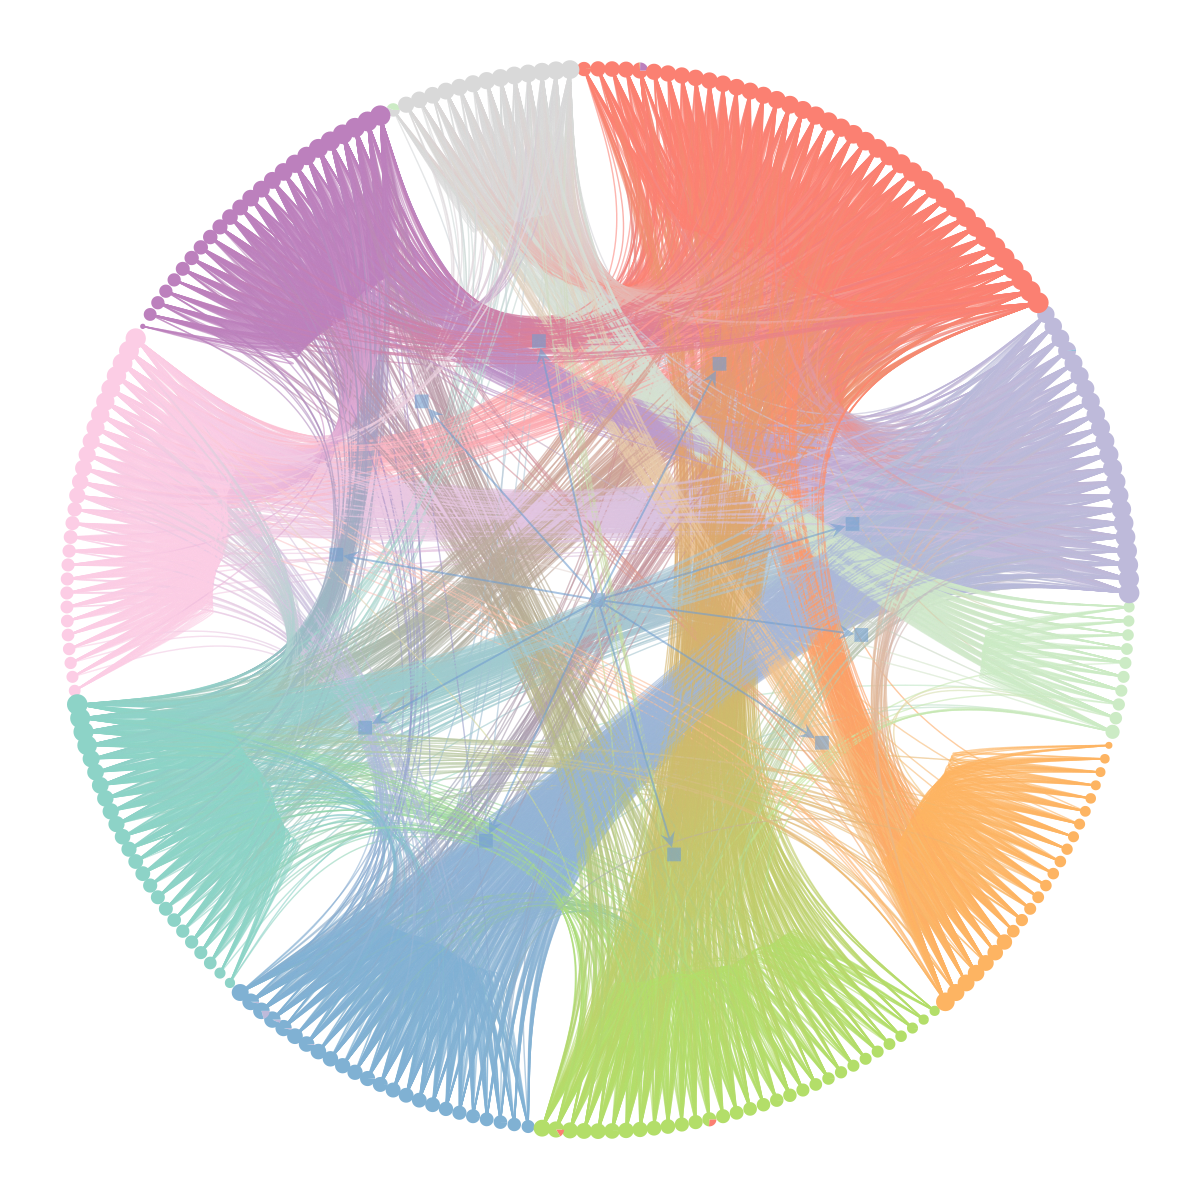
\includegraphics[width=0.28\linewidth]{img/school-graph.png}
	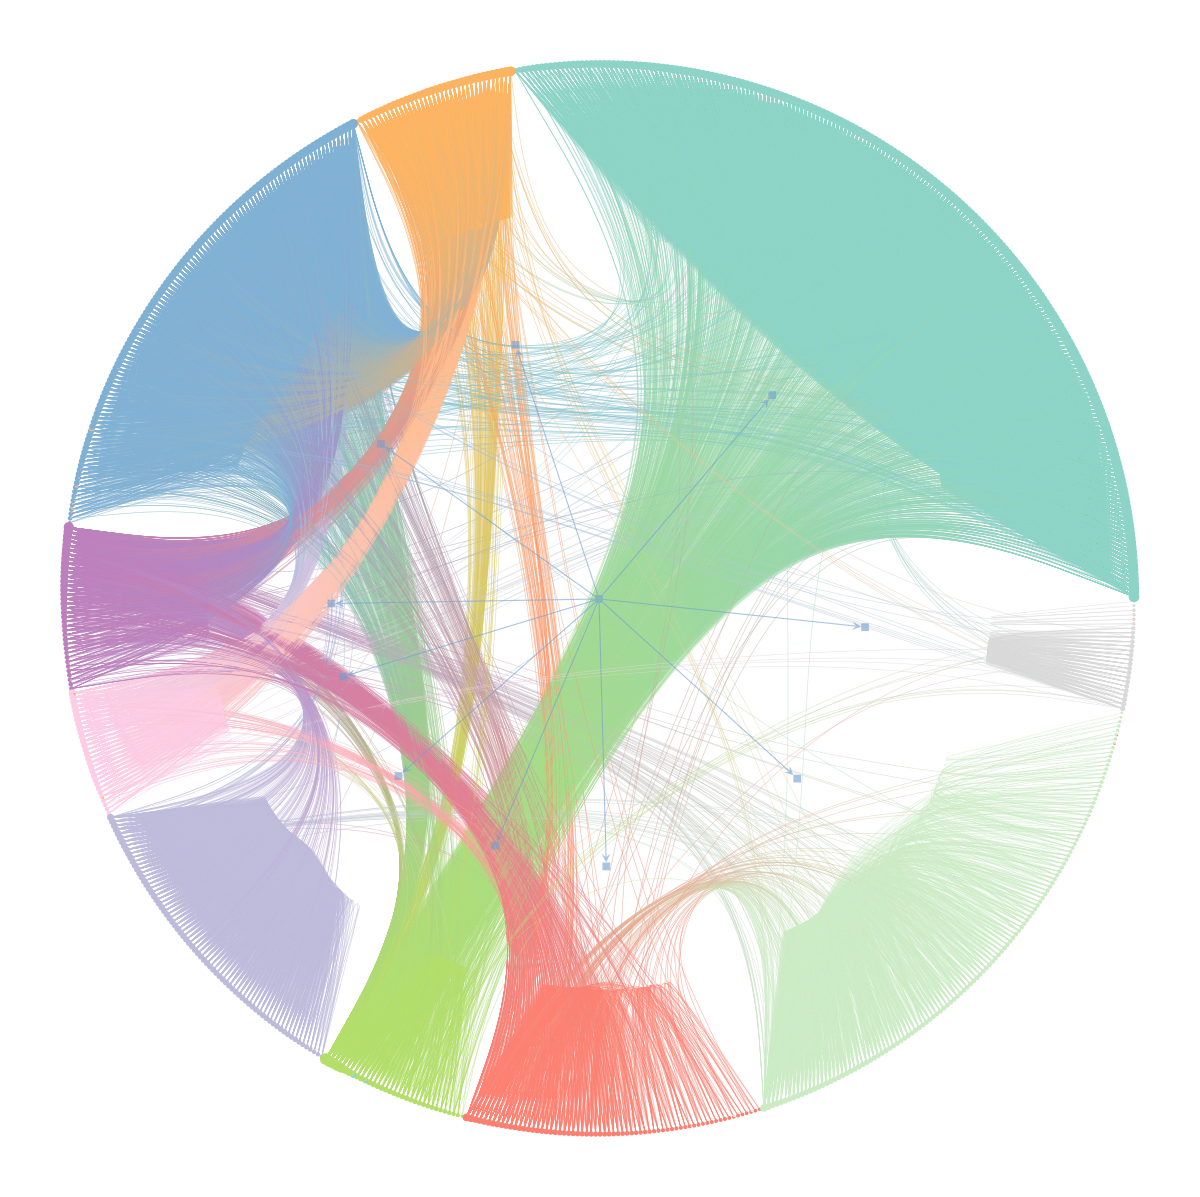
\includegraphics[width=0.28\linewidth]{img/fb-graph.png}
	\caption{Networks laid out and coloured according to inferred block memberships. Left to right: Polbooks, Krebs (2004); Primary School, Stehle et al (2011); Facebook Egonet, Leskovec and Mcauley (2012).}
	\label{fig:graphs-all}
\end{figure}


	\section{Conclusion}
\label{sec:conclusion}

The feature-first block model
(FFBM) is introduced, as a 
new generative model for labelled 
networks with communities.
An efficient MCMC algorithm  
is developed for sampling 
from the posterior distribution of
the relevant parameters in the FFBM;
the main idea is to divide up the graph into 
its most natural partition under the associated
parameter values, and then to determine whether 
the vertex features can accurately explain the partition. 
Through applications on empirical
network data, this approach 
is demonstrated to be effective at extracting and describing 
the most natural communities in a labelled network. 
Nevertheless, it
can only currently explain the structure at the macroscopic
scale. Future work will benefit from extending 
the FFBM to a further hierarchical model,
so that
the structure of the network 
can be explained at all scales of interest.



	
	\clearpage
	
	%references
	\bibliography{sources.bib}
	
	\clearpage
	\appendix
	
	\section{Additional material}

\subsection{SBM likelihood and prior}
\label{appdx:sbm}

For reference, we provide the likelihood and priors for the microcanonical SBM proposed by \citet{Peixoto-Bayesian-Microcanonical}. We have that the graph $A$ is drawn from the SBM,
%
\begin{equation}
	A \sim \textrm{DC-SBM}_{\textrm{MC}}(b, e, k),
\end{equation}
%
with edges placed uniformly at random but respecting the constraints imposed by $b, e$ and $k$. The computation of the likelihood, $p(A|k, e, b)$, is simply a case of counting the number of configurations that yield the same adjacency matrix and dividing by the total number of configurations possible. This is what gives this formulation the `microcanonical' moniker. If we consider the half-edges to be distinguishable for a moment, the total number of configurations that satisfy the $e$ constraint is,
%
\begin{equation}
	\Omega(e) = \frac{\prod_{r} e_r !}{\prod_{r,s : r < s} e_{rs}! \cdot \prod_{r} e_{rr}!!},
\end{equation}
%
where $e_r \coloneqq \sum_{s} e_{rs}$ and $(2m)!! \coloneqq 2^m m!$. Nevertheless, a great number of these $\Omega(e)$ total configurations yield the same graph $A$. We denote the number of configurations that yield the adjacency matrix $A$ with,
%
\begin{equation}
	\Xi(A) \coloneqq \frac{\prod_i k_i !}{\prod_{i,j : i < j} A_{ij} ! \prod_i A_{ii} !! }.
\end{equation}
%
Note the similarity between the forms of $\Omega(e)$ and $\Xi(A)$ as $e$ is effectively the adjacency matrix of the block-graph. With these defined we can write the overall likelihood as the ratio of the two:
%
\begin{equation}
	p(A|k,e,b) = \frac{\Xi(A)}{\Omega(e)}.
\end{equation}
%
Obviously, this form is only defined if $A$ respects the constraints imposed by $(k,e,b)$ else the likelihood is 0. 

With the likelihood defined, we turn our attention to the prior, necessary for Bayesian analysis. As discussed in the main text, the block membership vector $b$ is an intermediate variable in the FFBM so we are not free to choose a prior for it. Nevertheless, we can define the prior on $(e,k)$ as a conditional on $b$. We switch back to the FFBM notation of $\psi = \{\psi_e, \psi_k\}$ to encapsulate $e$ and $k$. We recall for reference
the prior $p(\psi | b)$ from \cite{Peixoto-Bayesian-Microcanonical}:
%
\begin{equation}
	p(\psi_e=e, \psi_k=k | b) = p(e | b) p(k | e, b) = \left[ \specialchoose{ \specialchoose{B}{2} }{ E} \right]^{-1} 
	\cdot \left[ \prod_r \frac{\prod_j \eta_j^r !}{n_r! q(e_r, n_r)} \right],
\end{equation}
%
where $\specialchoose{n}{m}$ is shorthand 
for $\binom{n+m-1}{m} = \frac{(n+m-1)!}{(n-1)!(m)!}$,
which can be thought of as the total number of distinct histograms 
produced by $m$ samples in $n$ bins.
The value
$E = \frac{1}{2} \sum_{r,s} e_{rs}$ is the total number of edges in the graph. 
Importantly, $E$ is not allowed to vary and so $p(e|b)$ is uniform in $e$.
The variable $\eta_j^r$ denotes the number of vertices in block $r$ 
that have degree $j$; formally, $\eta_j^r \coloneqq \sum_{i} \one\left\{b_i = r \right\} \one \left\{k_i = j \right\}$. 
The denominator $q(m, n)$ denotes the number of different histograms 
produced by $m$ samples in 
at most $n$ non-zero bins that sum to $m$. 
Finally, $e_r \coloneqq \sum_{s} e_{rs}$ is the total number 
of half edges in block $r$ and $n_r \coloneqq \sum_{i} \one\{b_i = r\}$ 
is the number of vertices assigned to block $r$. 

These priors were chosen carefully in \cite{Peixoto-Bayesian-Microcanonical} to 
more closely match the structure of empirical networks than simple 
uniform priors. We do not repeat these arguments here.

\subsection{Choosing the MALA step-size}
\label{appdx:step-size}

Recall that in 
Section~\ref{s:sfb} we used 
the Metropolis-adjusted Langevin algorithm (MALA)
to 
sample from the $\theta$-chain of the block membership 
generator parameters.
At iteration $t$, the proposed sample is generated by:
%
\begin{equation}
	\theta' = \theta^{(t)} - h_t \nabla U(\theta^{(t)}) + \sqrt{2h_t} \cdot \xi.
\end{equation}
%
There are two competing objectives when choosing the step-size $h_t$. 
On the one hand, $h_t$ needs to be large so that the sampler
arrives at a high density region quickly,
while too large a step-size would lead to low acceptance rates and thus 
inefficient sampling. An effective strategy is
to use {\em simulated annealing}: allow $h_t$ to slowly decrease
with $t$, as long as $h_t>0$ for all $t$ and also:
%
\begin{equation}
	\sum_{t=1}^{\infty} h_t = \infty, \qquad \textrm{and} \qquad
	\sum_{t=1}^{\infty} h_t^2 < \infty.
	\label{eqn:h-constraints}
\end{equation}
%
Following \citet{Bayesian-SGLD}, we adopt the 
polynomially decaying step-sizes,
%
$h_t = \alpha(\beta + t)^{-\gamma}$,
%
where $\alpha>0$, $\beta>0$ and $\gamma\in(1/2,1]$ are hyper-parameters.
We make the specific choices,
%
\begin{equation}
	\alpha = \frac{250 \cdot s}{N}, \qquad \beta = 1000, \qquad \gamma = 0.8,
	\label{eqn:step-size-params}
\end{equation}
%
where $N$ is the number of data-points and $s$,
the {\em step-size scaling}, is the only free parameter.

As an aside, we note that an interesting modification to MALA can be made if we skip out the Metropolis-Hastings accept/reject step entirely. If this is done, the algorithm is instead called the stochastic gradient Langevin dynamics (SGLD) \cite{Bayesian-SGLD}. This speeds up computation at the expense of the exactness of the method. Indeed, it relies on the fact that as the step-size is annealed to 0, the acceptance probability gets close to 1. Figure \ref{fig:step-size-tradeoff} gives empirical backing to this approximate rule-of-thumb. Nevertheless, as SGLD is not exact, we only use MALA for experimentation.

In order to choose the exact value of the {\em step-size scaling} $s$ for each experiment, we must quantify the trade-off between acceptance ratio and burn-in time. We illustrate the adopted method using the primary school dataset \cite{schools} as an example. We run the $b$-chain for $T_b = 1,000$ iterations and subsample such that $\Tcal_b$ is computed with $\kappa_b=0.2$ and $\lambda_b=5$. We then use this to run the $\theta$-chain for $T_\theta = 10,000$ iterations. The acceptance ratio -- which we denote $r_\alpha$ -- is simply the fraction of proposed moves which we accept. However, to measure burn-in we define a new metric: the mean of the objective function averaged over all samples,
%
\begin{equation}
	\bar{U} \coloneqq \frac{1}{T_\theta} \sum_{t \in [T_\theta]} U\left( \theta^{(t)} \right).
\end{equation}
%
Since the chain will equilibrate in the vicinity of a minima in $U(\theta)$, the average over all samples is a rough indicator of the speed of burn-in. The higher the value of $\bar{U}$, the longer we infer the chain took to burn in and reach equilibrium. This method relies on the assumption that the random starting point $\theta^{(0)}$ has a high value for the objective function $U(\theta^{(0)})$; this assumption holds as the domain of $\theta$ is a high dimensional space so we are unlikely to get a low $U(\theta)$ from a lucky guess. We plot the acceptance ratio $r_\alpha$ and average objective $\bar{U}$ for $10$ values of the step-size multiplier $s$ logarithmically spaced in the range $(10^{-2}, 10^1)$ on Figure \ref{fig:step-size-tradeoff}.
%
\begin{figure}[!h]
	\centering
	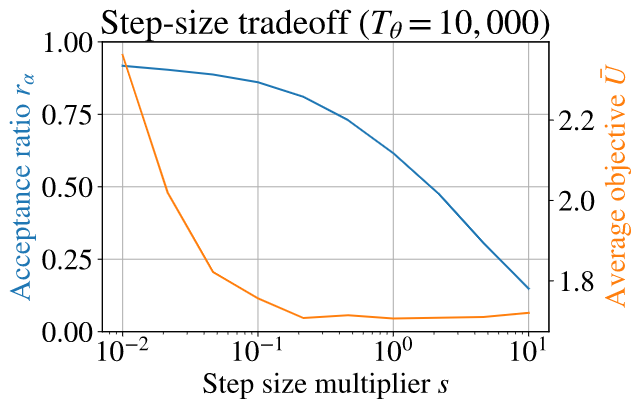
\includegraphics[width=0.6\linewidth]{step-size-tradeoff}
	\caption{Primary school dataset \cite{schools} illustration of step-size tradeoff}
	\label{fig:step-size-tradeoff}
\end{figure}

We see immediately that the acceptance ratio $r_\alpha$ steadily decreases with $s$. This is expected as large jumps for each proposal make it unlikely we stay in a high density region of our target distribution. A low acceptance ratio leads to wasted samples and is obviously undesirable.

Nevertheless, $\bar{U}$ decreases with $s$ indicating shorter burn-in times for larger step-sizes. However, this effect plateaus for $s>0.2$ for this particular dataset. Therefore, we choose $s=0.2$ as our step-size multiplier for the primary school dataset as this yields the best trade-off between $r_\alpha$ and $\bar{U}$. The step-sizes for the other datasets were chosen following the same argument but we do not repeat the process here.

\FloatBarrier
\subsection{Burn-in and thinning}
\label{appdx:burn-in-thinning}

%As with any MCMC method, we must deal with the issues presented by burn-in and thinning.
When sampling from the $b$ and $\theta$-chains described
in Section~\ref{sec:inference}, we respectively generate
$T_b$ and $T_\theta$ samples total.
We discard an initial proportion $\kappa_\star\in(0,1)$ of the samples 
as corresponding to a ``burn-in'' period required for the distribution 
of the chain to reach a distribution close to our target,
and we also ``thin'' the remaining samples to 
obtain a less-dependent version. For $\star\in\{b,\theta\}$,
the remaining sample sets are denoted $\Tcal_\star$
in the notation of Section~\ref{s:ss},
%
\begin{equation}
	\Tcal_\star = \{T_\star \kappa_\star + i \lambda_\star :  
	0 \leq i \leq \lfloor T_\star(1 - \kappa_\star) / \lambda_\star \rfloor \},
\end{equation}
%
where $\lambda_\star$ controls the thinning. The choice of
$\kappa_\star$ can be determined by plotting the log-target (either $S(b^{(t)})$ 
or $U(\theta^{(t)})$ as a function of $t$,
and choosing $\kappa_\star$ to encompass the region where the log-target has 
roughly reached equilibrium. As we do not leverage sample independence,
$\lambda_\star$ can be chosen less rigorously; we often simply
use $\lambda_b=5$ and $\lambda_\theta = 10$.

By way of illustration, we can consider the primary school dataset \cite{schools}. We plot the normalised objective function $U\left( \theta^{(t)} \right) / N$ with respect to MALA iteration on Figure \ref{fig:school-U-orginal} -- using the hyperparameters given in Appendix \ref{appdx:hyperparams}. We see that the chain converges to the modal neighbourhood quickly (within about 2000 iterations of a total 10,000). Nevertheless, we pick $\kappa_\theta=0.4 > 0.2$ to be on the safe-side. $\lambda_\theta=10$ is chosen somewhat arbitrarily as we do not require neighbouring samples to be independent. However, this thinning also has the advantage of speeding up computation of quantities that require an average over all the retained samples -- as $|\Tcal_\theta| < T_\theta$.
%
\begin{figure}[!h]
	\centering
	\begin{subfigure}[t]{0.4\linewidth}
		\centering
		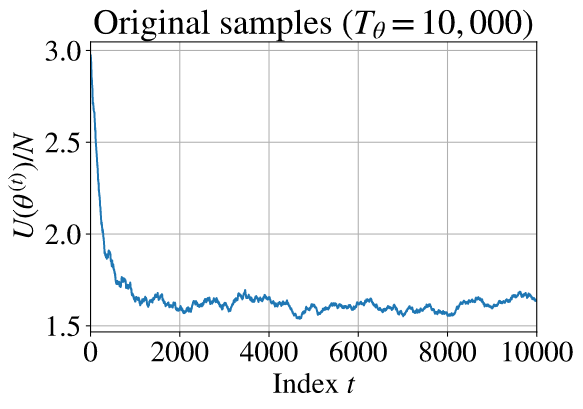
\includegraphics[width=\linewidth]{school-U-original.png}
		\caption{Original samples $t \in [T_\theta]$}
		\label{fig:school-U-orginal}
	\end{subfigure}
	\begin{subfigure}[t]{0.4\linewidth}
		\centering
		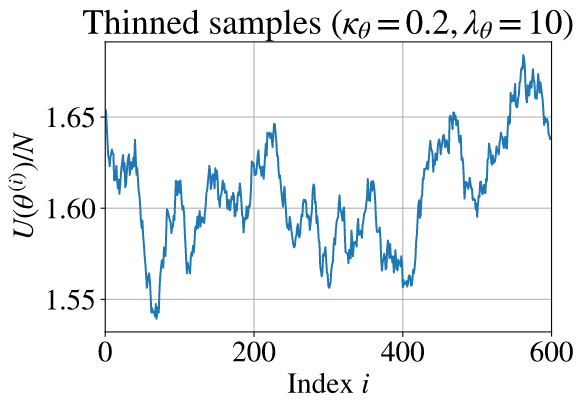
\includegraphics[width=\linewidth]{school-U-thinned.png}
		\caption{Thinned samples $t \in \Tcal_\theta$ indexed by $i$}
		\label{fig:school-U-thinned}
	\end{subfigure}
	\hspace{1cm}
	\caption{Primary school dataset normalised objective function against sample index}
\end{figure}

We plot the retained samples on Figure \ref{fig:school-U-thinned}. $U(\theta^{(i)})/N$ does bounce around a small amount but this is expected as we are sampling from the posterior rather than converging to the MAP solution. There does appear to be variation over a long time-scale but this is acceptable as we do not strictly require sample independence.
\FloatBarrier
\subsection{Initializing the b-chain}

For the purposes of the FFBM model, the number of blocks $B$ is a constant 
which must be specified. If the choice of $B$ is influenced 
by the observed data, then the analysis is no longer ``fully Bayesian''
and belongs to the class of methods referred to as ``empirical Bayes.''
However, as the number of blocks only specifies the coarseness of the 
analysis, it is reasonable to allow it to vary. Indeed, 
\citet{peixoto-determine-B} shows that for a fixed 
average degree the maximum number of detectable blocks scales 
as $O(\sqrt{N})$ where $N$ is the number of vertices.

If $B$ is allowed to vary in the $b$-chain (i.e.,
when new blocks can be created and empty blocks are allowed),
then the chain can be run until a minimum description 
length (MDL) solution is reached. We take the number of non-empty blocks 
in the MDL solution to be our fixed block number $B$ for subsequent analysis. 
Indeed, it is prudent to start the $b$-chain at this MDL solution as then 
the necessary burn-in time can be greatly reduced.

\subsection{Dimensionality discussion}
\label{appdx:dimension}

Many vertex feature often take only one of several discrete values within a set. For example, with the primary school dataset \cite{schools}, a pupil's school-class can take one of 10 values from \{``1A", ``1B", ``2A", ``2B" \dots ``5A", "5B"\}.

It is not immediately obvious how to encode this for the feature-to-block classifier. Although this is technically only a single dimension, we choose to expand the data into a set of 10 binary feature flags all taking values in the set $\Xcal = \{0, 1\}$. Although only one flag will be set at a time it is the simplest method for representing discrete-valued data. The reason we choose $\Xcal=\{0, 1\}$ and not $\Xcal = \{-1, 1\}$ is that the former allows for simpler analysis of the resulting weight values; when a feature $d$ is switched off then $x_{d}=0$ given $\Xcal = \{0, 1\}$, and the feature has no impact on the softmax output. This would not be the case for $\Xcal = \{-1, 1\}$.

Furthermore, it is more intuitive to only model positive relationships. In other words, we prefer to say that this block is comprised of the vertices with feature $d$ turned on rather than this block contains the vertices with feature $d$ switched off. To summarise the approach explicitly, say we have a feature encoding a pupil's gender: \{"male", "female"\}, we represent this as 2 binary feature flags "male": \{0, 1\} and "female": \{0, 1\}. This approach may seem inefficient but it is vital to ensure we can interpret the resulting parameter distributions.

Nevertheless, this dimensionality expansion means that we should not include a bias term in our softmax as then the MAP solution is less peaked and our $\theta$-samples will have higher variance. To illustrate this point we need only look at the form of the softmax activation function with bias vector $\beta$, operating on a vector $x$ which only has one non-zero entry $x_d=1$. Component $j$ of the output is given by:
%
\begin{equation}
	\phi_j(x) = \frac{\exp(w_j^T x + \beta_j)}{\sum_{k \in [B]} \exp(w_k^T x + \beta_k)} = 
	\frac{\exp(w_{jd} + \beta_j)}{\sum_{k \in [B]} \exp({w_{kd} + \beta_k})}.
	\label{eqn:softmax-bias}
\end{equation}
%
The term $w_{kd} + \beta_k$ is effectively the new weight for component $k$ as these two terms will always appear together. The bias term $\beta_k$ is therefore an unnecessary extra degree of freedom. To illustrate this point, we set $\beta_k=\beta_0$ for all $j$. If this is the case then equation \ref{eqn:softmax-bias} can be simplified to:
%
\begin{equation}
	\phi_j(x) = \frac{\exp(\beta_0) \cdot \exp(w_{jd})}{\sum_{k \in [B]} \exp(\beta_0) \cdot \exp(w_{kd})}
	= \frac{\exp(w_{jd})}{\sum_{k \in [B]} \exp(w_{kd})}
\end{equation}
%
This expression is independent of $\beta_0$ and so it is free to vary. This is not the whole picture as we also have the prior which introduces a regularisation term which favours weights closer to 0. This ensures the MAP solution is unique. Nevertheless, for mutually exclusive binary feature flags, the bias term does not add to the expressiveness of the model and only serves to complicate analysis. We therefore remove the bias term from the softmax.

Even for data comprised of several feature-classes each expanded into flags (e.g. school class and gender) we prefer to discard the bias term. The bias term only serves to decrease the objective function by leveraging information about the size of each detected block and not feature information. We do not wish to be overly confident in our block predictions when such predictions are influenced by block size and not feature information. Indeed, the approach was initially developed with a bias term but we found its removal yielded more reliable and reproducible results.

\subsection{Hypothesis test on feature weights}
\label{appdx:hyp-test}

We are given samples $\{\theta^{(t)}\}_{t \in \Tcal_\theta} \sim p(\theta | A, X)$ and wish to determine the statistical significance of the weights. We adopt matrix notation for simplicity by representing $\theta$ with the matrix $B \times D$ matrix of feature weights $W$. The question is to determine the significance of a particular feature $d$ by examining the value of $W_{id}$ for all the values $i \in [B]$. We know that the posterior is proportional to the prior multiplied by the likelihood,
%
\begin{equation}
	p(\theta|A, X) \propto p(\theta) \cdot p(A | \theta, X),
\end{equation}
%
assuming that the feature matrix $X$ is already given. The prior term can be evaluated but the likelihood is intractable. The closest we can get is through a Monte-Carlo integration over $b$,
%
\begin{align}
	p(A | \theta, X) &= \sum_{b \in [B]^N} p(A, b | \theta, X) \nonumber \\
	&= \sum_{b \in [B]^N} p(A | b, \theta, X) \cdot p(b | \theta, X) \nonumber \\
	&= \sum_{b \in [B]^N} p(A | b) \cdot p(b | \theta, X) \nonumber \\
	&\approx \sum_{i} p\left( A | b^{(i)} \right) \quad \textrm{with} \quad b^{(i)} \sim p(b| \theta, X).
	\label{eqn:mc-likelihood}
\end{align}
%
This could be implemented for a single value of $\theta$ but such a form cannot be used to characterise the overall form of the posterior. Nevertheless, the form in~(\ref{eqn:mc-likelihood}) highlights something interesting. The likelihood is peaked around areas of $\theta$ that generate a partition $b$ that is highly likely in the SBM sense -- high $p(A|b)$. This provides the motivation for using the Laplace approximation for modelling the posterior $p(\theta | A, X) \approx p(\theta; \hat{\mu}, \hat{\Sigma})$; we use a multivariate Gaussian to approximate the posterior. Indeed, the Laplace approximation is often used for modelling the posterior in logistic classification \cite{laplace}. This approximation is not exact but it motivates the derivation of the dimensionality reduction technique we construct by analogy with hypothesis testing. Marginalising over the other elements, the posterior for each element of the weight matrix $W$ can be approximated by,
%
\begin{equation}
	p(W_{ij}|A, X) \approx \Gaussian(W_{ij}|\hat{\mu}_{ij}, \hat{\sigma}_{ij}^2).
\end{equation}
%
Where we have used the set of samples for $W$ drawn according to the exact posterior, to calculate unbiased estimates for the mean and standard deviation:
%
\begin{equation}
	\hat{\mu}_{ij} \coloneqq \frac{1}{|\Tcal_\theta|} \sum_{t \in \Tcal_\theta} W_{ij}^{(t)} \qquad \textrm{and} \qquad
	\hat{\sigma}_{ij}^2 \coloneqq \frac{1}{|\Tcal_\theta|} \sum_{t \in \Tcal_\theta} \left( W_{ij}^{(t)} - \hat{\mu}_{ij} \right)^2.
\end{equation}
%
This approximation is not exact but we can show it is accurate empirically. Indeed, if we run the primary school experiment with hyper-parameters given in Appendix \ref{appdx:hyperparams}, we can then plot histograms of the collected $W$-samples and compare these to the Laplace approximation. The results are given on Figure \ref{fig:school-histogram}. Even though the Laplace approximation is not exact, it is remarkably reliable. 

\begin{figure}[!h]
	\centering
	\begin{subfigure}[t]{0.32\linewidth}
		\centering
		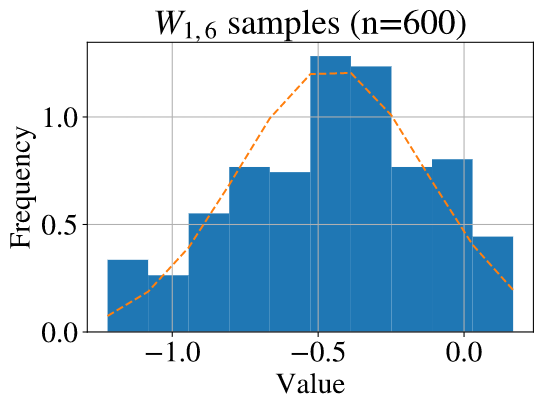
\includegraphics[width=\linewidth]{school-sample-histogram-16.png}
		\caption{Weight for block 1, class 3B}
	\end{subfigure}
	\hfill
	\begin{subfigure}[t]{0.32\linewidth}
		\centering
		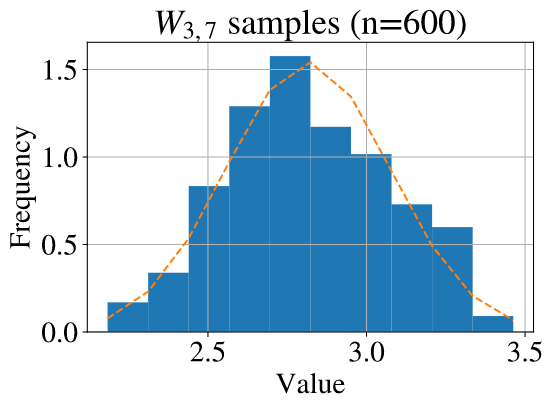
\includegraphics[width=\linewidth]{school-sample-histogram-37.png}
		\caption{Weight for block 3, class 4A}
	\end{subfigure}
	\hfill
	\begin{subfigure}[t]{0.32\linewidth}
		\centering
		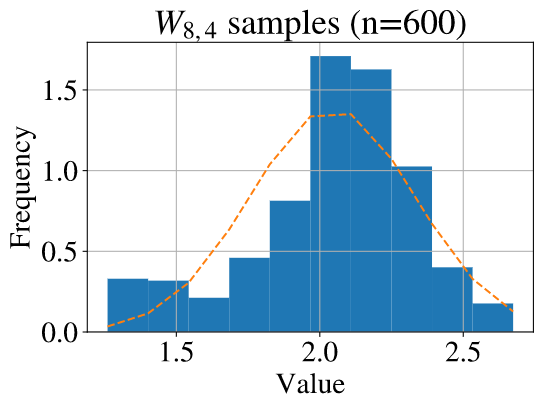
\includegraphics[width=\linewidth]{school-sample-histogram-84.png}
		\caption{Weight for block 8, class 2B}
	\end{subfigure}
	
	\caption{Histograms of sampled weights for the primary school experiment \cite{schools}. Dotted line is the applied Laplace approximation.}
	\label{fig:school-histogram}
\end{figure}

Using the approximation, we wish to construct a test to determine whether a particular weight value has $|W_{ij}| > c$ with high probability, where $c>0$. More specifically, we wish to decide between:
%
\begin{equation}
	\begin{aligned}
		H_0&: |W_{ij}| \leq c \\
		H_1&: |W_{ij}| > c
	\end{aligned}
\end{equation}
%
We can consider the probabilities $p(W_{ij} > c)$ and $p(W_{ij} < c)$ separately. Starting with $p(W_{ij} > c)$, we write this as,
%
\begin{align*}
	p(W_{ij} > c) &= p\left(Z > \frac{c - \hat{\mu}_{ij}}{\hat{\sigma}_{ij}}\right) \\
	&= p\left(-Z < \frac{\hat{\mu}_{ij} - c}{\hat{\sigma}_{ij}}\right)\\
	&= \Phi\left(\frac{\hat{\mu}_{ij} - c}{\hat{\sigma}_{ij}}\right),
\end{align*}
%
where $Z \sim \Gaussian(0,1)$ and $\Phi(\cdot)$ is the standard Gaussian cumulative density function. We introduce the variable $k$ to control the degree of significance of the result. Enforcing $k$ to be less than the argument of $\Phi$ gives us that: 
%
\begin{equation*}
	\hat{\mu}_{ij} - k \hat{\sigma}_{ij} > c.
\end{equation*}
%
As $\Phi(\cdot)$ is monotonically increasing, this yields the following:
%
\begin{equation}
	p(W_{ij} > c) > \Phi(k) \iff \hat{\mu}_{ij} - k \hat{\sigma}_{ij} > c.
	\label{eqn:hyp-test-positive}
\end{equation}
%
A similar argument can be made to show that:
%
\begin{equation}
	p(W_{ij} < -c) > \Phi(k) \iff \hat{\mu}_{ij} + k \hat{\sigma}_{ij} < -c.
	\label{eqn:hyp-test-negative}
\end{equation}
%
Clearly equations \ref{eqn:hyp-test-positive} and \ref{eqn:hyp-test-negative} cannot both hold simultaneously as $c, \hat{\sigma}_{ij}, k>0$. Nevertheless, a necessary and sufficient condition for one of them to hold is:
%
\begin{equation}
	(\hat{\mu}_{ij} - k \hat{\sigma}_{ij}, \hat{\mu}_{ij} + k \hat{\sigma}_{ij}) \cap (-c, +c) = \emptyset
	\label{eqn:hyp-test-empty}
\end{equation}
%
This is equivalent to saying that $\hat{\mu}_{ij}$ is at least $k$ standard deviations away from the range $(-c, c)$. We choose to reject the null hypothesis $H_0$ if and only if equation \ref{eqn:hyp-test-empty} holds. We can say with probability greater than or equal to $\Phi(k)$ that either $W_{ij} < -c$ or $W_{ij} > c$ thus rejecting the null $H_0: |W_{ij}| \leq c$.

Note that we choose to accept $H_0$ even in the case that the combined probabilities of $p(W_{ij} < -c) + p(W_{ij} > c) > \Phi(k)$, if equation \ref{eqn:hyp-test-empty} is not satisfied. This is because we wish to apply this for dimensionality reduction purposes. We only want to keep weights for which we have a confident prediction outside the range $(-c, c)$ not those that succeed by summing the two extremes of their distribution. Note that this case is very rare empirically but it nonetheless must be specified.
	\clearpage
	
	\section{Appendix: Derivations}

\subsection{Derivation of conditional block distribution given feature matrix}
\label{appdx:b|x}

We wish to determine the form of $p(b| X)$. This can be done by integrating over the joint probability with respect to $\theta$.
%
\begin{align*}
	p(b | X) &= \int p(b , \theta| X, \theta) d\theta = \int p(b | X, \theta) p(\theta | X) d\theta \\
	&=\int p(b | X, \theta) p(\theta) d\theta = \int \prod_{i \in [N] } \phi_{b_i}(x_i; \theta) p(\theta) d\theta \\
	&= \prod_{i \in [N]} \int \frac{\exp(w_{b_i}^T \tilde{x}_i) \prod_{j \in [B]} \Gaussian(w_j; 0, \sigma_\theta^2 I)}{\sum_{k \in [B]} \exp(w_{k}^T \tilde{x}_i)} dw_{1:B}
\end{align*}
%
We note that $b_i \in [B]$ and so the integral's value is unchanged with respect to $b_i$. The integrand has the same form no matter which value $b_i$ takes as the prior is the same for each $w_j$. As such the integral can only be a function of at most $\tilde{x}_i$ and $\sigma_\theta^2$ as it is symmetric with respect to $b_i$ and all the various $w_j$ are integrated out as they are dummy variables. Therefore, denoting the integral by the (unknown) function $f(\tilde{x}_i, \sigma_\theta^2)$, we write $p(b| X)$ as follows:
%
\begin{align*}
	p(b | X) &= \prod_{i=1}^{N} f(\tilde{x}_i, \sigma_\theta^2) = \textrm{const w.r.t } b = c
\end{align*}
%
As this is a constant with respect to $b$ we conclude that $p(b | X)$ must be a uniform distribution. $\nicefrac{1}{c}$ is simply the size of the set of values that $b$ can take. We know $b_i \in [B]$. Therefore, $b \in [B]^N$ and $|[B]^N| = B^N = \nicefrac{1}{c}$. Putting this all together we conclude that:
%
\begin{equation}
	p(b | X) = B^{-N}
\end{equation}

\subsection{Derivation of U form}
\label{appdx:form-U}

The invariant distribution we wish to target for the $\theta$ samples is the posterior of $\theta$ given the values of the pair $(X, b)$. We write this as follows:
%
\begin{align}
	\pi_\theta(\theta) &\propto p(\theta | X, b) \propto p(b | X, \theta) p(\theta) \propto  \exp \left( - U(\theta) \right) \\
	\therefore U(\theta) &= - \left( \log p(b | X, \theta) + \log p(\theta) \right) + \textrm{const}
\end{align}
%
Where we have introduced $U(\theta)$ equal to the negative log posterior. Each of the constituent terms of $U(\theta)$ are easily computed (equation \ref{eqn:U-constituent-terms}) by defining $y_{ij} \coloneqq \one \left\{ b_i = j \right\}$ and $a_{ij} \coloneqq \phi_j(x_i; \theta)$.
%
\begin{equation}
	\log p(b | X, \theta) = \sum_{i \in [N]} \sum_{j \in [B]} y_{ij} \log a_{ij}  \quad \textrm{and} \quad
	\log p(\theta) = -\frac{(D+1)(B)}{2} \log 2\pi - \frac{1}{2 \sigma_\theta^2} || \theta ||^2
	\label{eqn:U-constituent-terms}
\end{equation}
%
Discarding constant terms, we write $U(\theta)$ as in equation \ref{eqn:U-form-appdx-0}. Note that $||\theta||^2 = \sum_{i} \theta_{i}^2 = \sum_{j=1}^{B} ||w_j||^2$ is the Euclidean norm of the vector of parameters $\theta$.
%
\begin{equation}
	U(\theta) = \left( \sum_{i=1}^{N} \sum_{j=1}^{B} y_{ij} \log \frac{1}{a_{ij}} \right)
	+ \frac{1}{2\sigma_\theta^2} ||\theta||^2 = N \cdot \Lcal(\theta) + \frac{1}{2\sigma_\theta^2} ||\theta||^2
	\label{eqn:U-form-appdx-0}
\end{equation}
%

\subsection{Derivation of U gradient with respect to feature parameters}
\label{appdx:gradu}
The goal is to determine $\nabla U(\theta)$, the gradient of the negative log posterior with respect to the parameters. We repeat the form of $U(\theta)$ in equation \ref{eqn:U-form-appdx}.
%
\begin{equation}
	U(\theta) = \left( \sum_{i \in [N]} \sum_{j \in [B]} y_{ij} \log \frac{1}{a_{ij}} \right)
	+ \frac{1}{2\sigma_\theta^2} ||\theta||^2
	\label{eqn:U-form-appdx}
\end{equation}
%
Where $y_{ij}$ is independent of $\theta$ and $a_{ij}$ is the output from the softmax layer, with form as given in equation \ref{eqn:a-ij}.
%
\begin{equation}
	a_{ij} \coloneqq \phi_{j} (x_i; \theta) = \frac{\exp(w_j^T \tilde{x}_i)}{\sum_{r \in [B]} \exp(w_r^T \tilde{x}_i)}
	\label{eqn:a-ij} 
\end{equation}
%
We note that $\theta = \{w_k\}_{k=1}^B$, and as such we can write this in vector form $\theta = \left[w_1^T, w_2^T \dots w_B^T  \right]^T$. Therefore, $\nabla U(\theta) = \left[\nicefrac{\partial U}{\partial w_1}^T,\nicefrac{\partial U}{\partial w_2}^T \dots \nicefrac{\partial U}{\partial w_B}^T  \right]^T$; to compute $\nabla U(\theta)$ it suffices to find the form of $\nicefrac{\partial U}{\partial w_k}$ with respect to a general $k$.

To this end, we must first find partial derivatives of $a_{ij}$ and $||\theta||$ with respect to $w_k$. Starting with $a_{ij}$:
%
\begin{align}
	\frac{\partial a_{ij}}{\partial w_k} &= \frac
	{\tilde{x}_i \exp(w_j^T \tilde{x}_i) \delta_{jk} \cdot \sum_{r \in [B]} \exp(w_r^T \tilde{x}_i) 
		- 
		\exp(w_j^T \tilde{x}_i) \cdot \tilde{x}_i \exp(w_k^T \tilde{x}_i)}
	{\left( \sum_{r \in [B]} \exp(w_r^T \tilde{x}_i) \right)^2} \nonumber \\
	&= \tilde{x}_i \left( a_{ij} \delta_{jk} - a_{ij}a_{ik} \right) 
\end{align}
%
Where $\delta_{jk} \coloneqq \one \left\{ j = k \right\}$. Now moving onto the derivative of $||\theta||^2$:
%
\begin{equation}
	\frac{ \partial}{\partial w_k} ||\theta||^2 = \frac{\partial}{\partial w_k} \left( \sum_{r \in [B]} ||w_r||^2 \right) = 2w_k
\end{equation}
%
We are ready to put this all together, to find the partial derivative of $U(\theta)$ with respect to each $w_k$:
\begin{align}
	\frac{\partial U}{\partial w_k} &= 
	\sum_{i=1}^{N} \sum_{j=1}^{B} y_{ij} 
	\left( \frac{-\tilde{x}_i}{a_{ij}} \left( a_{ij} \delta_{jk} - a_{ij} a_{ik} \right) \right)
	+ \frac{w_k}{\sigma_\theta^2} \nonumber \\
	&=  - \left( \sum_{i=1}^{N} \tilde{x}_i \left( y_{ik} - a_{ik} \sum_{j=1}^{B} y_{ij} \right)
	- \frac{w_k}{\sigma_\theta^2} \right) \nonumber \\
	&= - \left( \sum_{i=1}^{N} \Big\{ \tilde{x}_i (y_{ik} - a_{ik}) \Big\} - \frac{w_k}{\sigma_\theta^2} \right)
\end{align}
%
This is the required result. This form can be computed efficiently through matrix operations. The only property of $y_{ij}$ we have used in the derivation is the sum-to-one constraint $\sum_{j=1}^{B} y_{ij} = 1$ for all $i$.

\subsection{Hypothesis test on feature weights}

We are given samples $\{\theta^{(t)}\}_{t \in \Tcal_\theta} \sim p(\theta | A, X)$ and wish to determine the statistical significance of the weights. We adopt matrix notation for simplicity by representing $\theta$ with the matrix $B \times D$ matrix of feature weights $W$. The question is to determine the significance of a particular feature $d$ by examining the value of $W_{id}$ for all the values $i \in [B]$. We know that the posterior is proportional to the prior multiplied by the likelihood (assuming that the feature matrix $X$ is already given):
%
\begin{equation}
	p(\theta|A, X) \propto p(\theta) \cdot p(A | \theta, X)
\end{equation}
%
The prior term can be evaluated but the likelihood is intractable. The closest we can get is through a Monte-Carlo integration over $b$:
%
\begin{align}
	p(A | \theta, X) &= \sum_{b \in [B]^N} p(A, b | \theta, X) \nonumber \\
	&= \sum_{b \in [B]^N} p(A | b, \theta, X) \cdot p(b | \theta, X) \nonumber \\
	&= \sum_{b \in [B]^N} p(A | b) \cdot p(b | \theta, X) \nonumber \\
	&\approx \sum_{i} p\left( A | b^{(i)} \right) \quad \textrm{with} \quad b^{(i)} \sim p(b| \theta, X)
	\label{eqn:mc-likelihood}
\end{align}
%
This could be implemented for a single value of $\theta$ but such a form cannot be used to characterise the overall form of the posterior. Nevertheless, the form in equation \ref{eqn:mc-likelihood} still does highlight something interesting. The likelihood is peaked around areas of $\theta$ that generate a partition $b$ that is highly likely in the SBM sense -- high $p(A|b)$. This provides the motivation for using the Laplace approximation for modelling the posterior $p(\theta | A, X) \approx p(\theta; \mu, \Sigma)$. Indeed, the Laplace approximation is often used for modelling the posterior in logistic classification \cite{laplace}. As a simplification we assume that $\Sigma$ is diagonal, therefore each element of $\theta$ is independent. This assumption does not hold in general but it motivates the derivation of the dimensionality reduction we construct by analogy with hypothesis testing. Assuming, $\Sigma$ is diagonal then the posterior for each element of the weight matrix $W$ can be approximated by:
%
\begin{equation}
	p(W_{ij}|A, X) \approx \Gaussian(W_{ij}|\hat{\mu}_{ij}, \hat{\sigma}_{ij}^2)
\end{equation}
%
Where we have used the set of samples for $W$ drawn according to the exact posterior, to calculate unbiased estimates for the mean and standard deviation:
%
\begin{equation}
	\hat{\mu}_{ij} \coloneqq \frac{1}{|\Tcal_\theta|} \sum_{t \in \Tcal_\theta} W_{ij}^{(t)} \qquad \textrm{and} \qquad
	\hat{\sigma}_{ij}^2 \coloneqq \frac{1}{|\Tcal_\theta|} \sum_{t \in \Tcal_\theta} \left( W_{ij}^{(t)} - \hat{\mu}_{ij} \right)^2
\end{equation}
%
This approximation is not exact but can show it is accurate empirically. Indeed, if we run the primary school experiment with hyper-parameters given in appendix \ref{appdx:hyperparams}, we can then plot histograms of the collected $W$-samples and compare these to the Laplace approximation. The results are given on figure \ref{fig:school-histogram}. Even though the Laplace approximation is not exact, it is remarkably reliable. 

\begin{figure}[!h]
	\centering
	\begin{subfigure}[t]{0.3\linewidth}
		\centering
		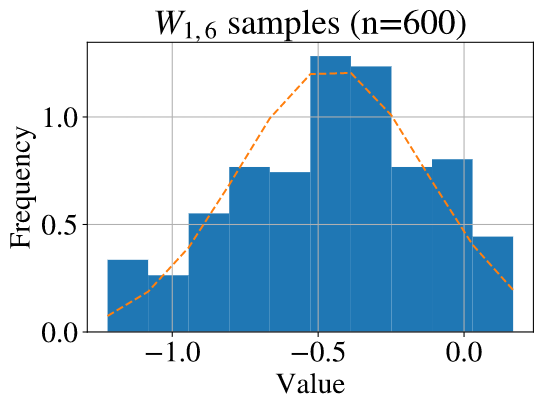
\includegraphics[width=\linewidth]{school-sample-histogram-16.png}
		\caption{Weight for block 1, class 3B}
	\end{subfigure}
	\hfill
	\begin{subfigure}[t]{0.3\linewidth}
		\centering
		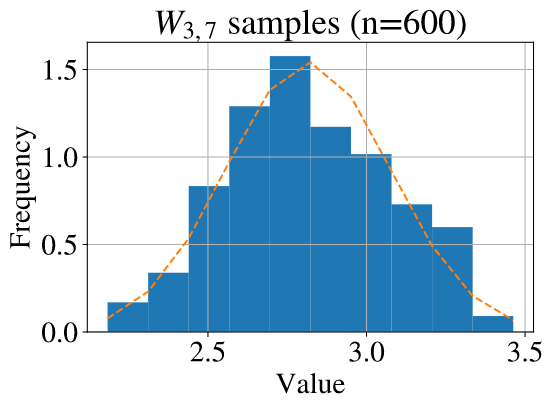
\includegraphics[width=\linewidth]{school-sample-histogram-37.png}
		\caption{Weight for block 3, class 4A}
	\end{subfigure}
	\hfill
	\begin{subfigure}[t]{0.3\linewidth}
		\centering
		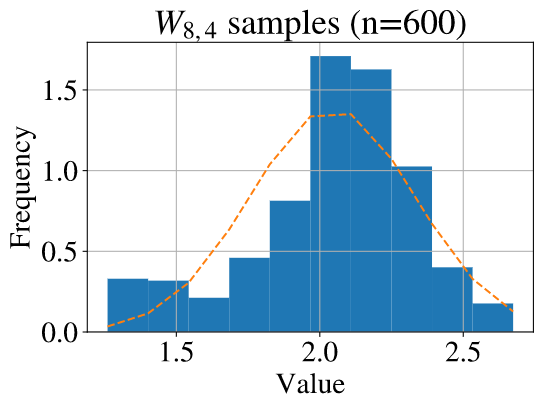
\includegraphics[width=\linewidth]{school-sample-histogram-84.png}
		\caption{Weight for block 8, class 2B}
	\end{subfigure}

	\caption{Histograms of sampled weights for the primary school experiment \cite{schools}. Dotted line is the applied Laplace approximation.}
	\label{fig:school-histogram}
\end{figure}

Using the approximation, we can construct a test to determine whether a particular weight value has $|W_{ij}| > c$ with high probability. Assuming without loss of generality that
%
\begin{equation}
	p(|W_{ij}| > c) = p(W_{ij})
\end{equation}
	\clearpage
	
	\section{Implementation details}

\subsection{Algorithms}
\label{appdx:algorithms}

\begin{algorithm} % enter the algorithm environment
	\caption{Block membership sample generation} % give the algorithm a caption
	\label{alg:b-samples} % and a label for \ref{} commands later in the document
	\begin{algorithmic} % enter the algorithmic environment
		\Procedure{SampleBlockMemberships}{$A, T_b$}
		\State $b^{(0)} \gets \argmin_b S(b|A)$ \Comment{Implemented as greedy heuristic in \textit{graph-tool} library}
		\For{$t \in \{0, 1 \dots T_b - 1\}$}
		\State $b' \gets \sim q_b(b^{(t)}, b' | A)$
		\State $\log \alpha_b \gets \log \alpha_b(b^{(t)}, b' | A)$
		\State $\eta \gets \sim \textrm{Unif}(0,1)$
		\If{$\log \eta < \log \alpha_b$}
		\State $b^{(t+1)} \gets b'$
		\Else
		\State $b^{(t+1)} \gets b^{(t)}$
		\EndIf
		\EndFor
		
		\State \textbf{return} $\{b^{(t)}\}_{t=1}^{T_b}$
		\EndProcedure
	\end{algorithmic}
\end{algorithm}

\begin{algorithm} % enter the algorithm environment
	\caption{FFBM parameter pseudo-marginal inference} % give the algorithm a caption
	\label{alg:theta-samples} % and a label for \ref{} commands later in the document
	\begin{algorithmic} % enter the algorithmic environment
		\Procedure{SampleFeatureWeights}{$X, \{b^{(t)}\}, \Tcal_b, \sigma_\theta, s$}
		\State $\hat{Y}_{ij} \gets \frac{1}{|\Tcal_b|} \sum_{t \in \Tcal_b} \one \{ b^{(t)}_i = j\} \quad \forall i,j$
		\State $\theta^{(0)} \gets \sim \Gaussian(0, \sigma_\theta I)$
		
		\item[]
		
		\For{$t \in \{0, 1 \dots T_\theta - 1\}$}
		\State $\xi \gets \sim \Gaussian(0, I)$
		\State $h_t \gets \frac{s}{N} \cdot 250(1000 + t)^{-0.8}$
		\State $g_t \gets \nabla U(\theta^{(t)}| X, \hat{Y})$
		\item[]
		\State $\theta' \gets \theta^{(t)} - h_t \cdot g_t + \sqrt{2h_t} \cdot \xi$
		\State $\log \alpha_\theta \gets \log \alpha_\theta(\theta^{(t)}, \theta' | A, \hat{Y})$
		\State $\eta \gets \sim \textrm{Unif}(0,1)$
		\If{$\log \eta < \log \alpha_\theta$}
		\State $\theta^{(t+1)} \gets \theta'$
		\Else
		\State $\theta^{(t+1)} \gets \theta^{(t)}$
		\EndIf
		\EndFor
		
		\State \textbf{return} $\{\theta^{(t)}\}_{t=1}^{T_\theta}$
		\EndProcedure
	\end{algorithmic}
\end{algorithm}

\begin{algorithm} % enter the algorithm environment
	\caption{Dimensionality reduction} % give the algorithm a caption
	\label{alg:retained-set} % and a label for \ref{} commands later in the document
	\begin{algorithmic} % enter the algorithmic environment
		\Procedure{ReduceDimension}{$\{W^{(t)}\}, \Tcal_\theta, k, D'$}
		
		\State $(B, D) \gets W^{(0)}$.shape
		\State $\hat{\mu}_{ij} \gets \frac{1}{|\Tcal_\theta|} \sum_{t \in \Tcal_\theta} W_{ij}^{(t)} \quad \forall i \in [B], j \in [D]$
		\State $\hat{\sigma}_{ij} \gets \frac{1}{|\Tcal_\theta|} \sum_{t \in \Tcal_\theta} \left( W_{ij}^{(t)} - \hat{\mu}_{ij} \right)^2 \quad \forall i \in [B], j \in [D]$
		
		\item[]
		
		\For{$d \in [D]$}
			\For{$i \in [B]$}
				\State $l_i \gets \hat{\mu}_{id} - k \cdot \hat{\sigma}_{id}$
				\State $u_i \gets \hat{\mu}_{id} + k \cdot \hat{\sigma}_{id}$
				\If{$l_i \leq 0$ and $u_i \geq 0$}
					\State $l_i, u_i \gets 0$
				\EndIf
			\EndFor
			\State $c_d \gets \max_i \min\left(|l_i|, |u_i| \right)$
		\EndFor
		
		\item[]
		
		\State indexArray $\gets$ indexSort($c$, descending=True)[$0:D'$]
		\State $d^* \gets$ indexArray[-1]
		\State $\Dcal' \gets $ Set(indexArray)
		\State $c^* \gets c_{d^*}$
		\State \textbf{return} $\Dcal', c^*$
		\EndProcedure
	\end{algorithmic}
\end{algorithm}

\FloatBarrier
\subsection{Hyperparameter values}
\label{appdx:hyperparams}

\begin{table}[!h]
	\centering
	\caption{Hyper-parameter values for each experiment}
	\label{tab:hyperparams}
	\resizebox{\textwidth}{!}{%
		\begin{tabular}{c|ccc|ccc|cccc|cc|cccc}
			Dataset & 
			$B$ & $f$ & $\sigma_\theta$ & 
			$T_b$ & $\kappa_b$ & $\lambda_b$ & 
			$T_\theta$ & $\kappa_\theta$ & $\lambda_\theta$ & $s$ &
			$k$ & $D'$ &
			$T_\theta'$ & $\kappa_\theta'$ & $\lambda_\theta'$ & $s'$
			\\ \hline
			Polbooks &
			3 & 0.7 & 1 &
			1,000 & 0.2 & 5 &
			10,000 & 0.4 & 10 & 0.05 &
			-- & -- & 
			-- & -- & -- & -- \\
			School &
			10 & 0.7 & 1 &
			1,000 & 0.2 & 5 &
			10,000 & 0.4 & 10 & 0.2 &
			1 & 10 & 
			10,000 & 0.4 & 10 & 0.2 \\
			FB Egonet &
			10 & 0.7 & 1 &
			1,000 & 0.2 & 5 &
			10,000 & 0.4 & 10 & 0.017 &
			1 & 10 & 
			10,000 & 0.4 & 10 & 0.5 \\
		\end{tabular}
	}
\end{table}

\subsection{Hardware specification}
\label{appdx:imp-details}

All data analysis and visualisation was implemented in Python. Full source code is available at:
\url{https://github.com/LozzaTray/Jormungandr-code}. A logbook was generated from the git commit history using the tool \href{https://github.com/Hugoagogo/pyGitBook}{pyGitBook} and is available as a separate file.
The scripts were run using a standard PC using the Windows Subsystem for Linux (WSL) environment. Specs are:

\begin{itemize}
	\item \textbf{CPU}: Intel(R) Core(TM) i7-1065G7
	\item \textbf{RAM}: 8GB
	\item \textbf{GPU}: Intel(R) Iris(R) Plus Graphics
\end{itemize}

On this hardware each experiment iteration took the following amount of time to execute:

\begin{table}[!h]
	\centering
	\caption{Compute-time for each experiment}
	\label{tab:compute-time}
	\begin{tabular}{c|ccc|c}
		Dataset & $b$-chain & $\theta$-chain & Reduced $\theta$-chain & Overall compute time \\ \hline
		Polbooks & $\sim$1s & $\sim$10s & -- & $\sim$11s \\
		School & $\sim$1s & $\sim$7s & $\sim$7s & $\sim$15s \\
		FB Egonet & $\sim$2s & $\sim$50s & $\sim$8s & $\sim$60s
	\end{tabular}
\end{table}


	%
	\clearpage
	\section{Risk assessment retrospective}

As experimental work was entirely computer-based, the risks encountered were not what one might typically associate with a more hands-on project: heavy machinery, dangerous chemicals etc. Most of the risks identified would be as a result of an improper working environment. These could be properly managed by ensuring the working environment felt comfortable. An external monitor went some way to alleviating the eye-strain of coding on a small screen for extended periods. Furthermore, an external mouse is far kinder on the wrist than a track-pad on laptops. There were no unexpected hazards encountered that were not identified at the start of the project.
	\section{Covid-19 disruption}

Please provide details of disrupted project work, including dates when the work was planned to take place and
reasons for the disruption (e.g. inaccessible equipment, illness).
If your work was disrupted, to what extent was it possible to redefine elements of your project so as to achieve
alternative goals? Please comment on the success, or otherwise, of the Covid-19 contingency plan that you
formulated last summer and documented on your Project Planning Form.
This appendix should not exceed one page in length.
	
\end{document}
